\documentclass[12pt,a4paper]{report}
\usepackage[utf8]{inputenc}
\usepackage[T1]{fontenc}
\usepackage{amsfonts}
\usepackage{setspace}
\usepackage{graphicx}
\usepackage{array}
\usepackage{fancyhdr}
\usepackage{geometry}
\usepackage{ragged2e}
\usepackage{color}
\usepackage{pdfpages}
\geometry{
    a4paper,
    left=1.15in,
    right=0.85in,
    top=1.0in,
    bottom=1.0in,
}
\usepackage{pdflscape}
\usepackage{float}
\usepackage{amsmath}
\usepackage{amssymb}
\usepackage{algorithm}
\usepackage{algorithmic}
\usepackage{longtable}
\usepackage{tikz}
\usepackage{rotating}
\usetikzlibrary{shapes,arrows,positioning,calc}
\usepackage{pgfplots}
\pgfplotsset{compat=1.18}


\begin{document}
\pagestyle{empty}
\begin{center}

{\large \textbf{Visvesvaraya Technological University, Belagavi - 590018}}
\begin{figure}[hbtp]
\centering

\includegraphics[width=2.3cm,height=2.8cm]{./pic/vtu}
\end{figure}

\textbf{PROJECT REPORT}
\par
\textbf{ON}
\par
\vspace{8pt}
{\Large\textbf{TransGraph-PPI: A Hybrid Ensemble Framework for
Sequence-Based Protein-Protein Interaction Prediction}}
\par
\vspace{10pt}
\par
\textit{\textbf{Submitted in partial fulfillment for the award of degree of }}
\par
\vspace{12pt}
\large \textbf{BACHELOR OF ENGINEERING }
\par
\textbf{in}
\par
\large \textbf{COMPUTER SCIENCE \& ENGINEERING}
\par
\vspace{12pt}
\textit{\textbf{Submitted by}}
\vspace{8pt}

\begin{center}
\begin{tabular}{l@{\hspace{2cm}}r}
\textbf{\large Ajay Preenal Dsouza} & \textbf{4SO23CS008} \\
\textbf{\large Ashwini Shenoy B} & \textbf{4SO23CS042} \\
\textbf{\large Basil S} & \textbf{4SO23CS050} \\
\textbf{\large Bhavish V} & \textbf{4SO23CS052} \\
\end{tabular}
\end{center}

\vspace{12pt}
\textit{\textbf{Under the Guidance of}}
\par
\vspace{6pt}
\textbf{Ms Jaishma Kumari B }
\par
\vspace{2pt}
\normalsize { Assistant Professor, Department of CSE }
\par
\begin{figure}[hbtp]
\centering

\includegraphics[scale=0.5]{./pic/sjeclogo}
\end{figure}
\large \textbf{DEPT. OF COMPUTER SCIENCE AND ENGINEERING}
\par \Large \textbf{ST JOSEPH ENGINEERING COLLEGE}
\par 
\textbf{An Autonomous Institution}
\par
{\large{(Affiliated to VTU Belagavi, Recognized by AICTE, Accredited by NBA)}}
\par
\vspace{3pt}
{\large \textbf{Vamanjoor, Mangaluru - 575028, Karnataka}}
\par 
\vspace{12pt}
{\large \textbf{2026-27}}
\end{center}
\newpage


% Certificate Page
\begin{center}
\LARGE \textbf{ST JOSEPH ENGINEERING COLLEGE}
\par
\Large \textbf{An Autonomous Institution}
\par \large{(Affiliated to VTU Belagavi, Recognized by AICTE, Accredited by NBA)}
\par \vspace{3pt}
\large \textbf{Vamanjoor, Mangaluru - 575028, Karnataka}
\par \vspace{12pt}  
\par
\large \textbf{DEPT. OF COMPUTER SCIENCE AND ENGINEERING}
\par
\begin{figure}[hbtp]
\centering

\includegraphics[scale=0.5]{./pic/sjeclogo}
\end{figure}


{\Large \textbf{CERTIFICATE}}
\end{center}
\justifying
\par
\setstretch{1.2}
\noindent 
Certified that the project work entitled \textbf{"TransGraph-PPI: A Hybrid Ensemble Framework for
Sequence-Based Protein-Protein Interaction
Prediction"} carried out by\vspace{0.25in} 
\par

\noindent 
\vspace{2pt} 
\begin{center}
\begin{tabular}{l@{\hspace{2cm}}r}
\textbf{\large Ajay Preenal Dsouza} & \textbf{4SO23CS008} \\
\textbf{\large Ashwini Shenoy B} & \textbf{4SO23CS042} \\
\textbf{\large Basil S} & \textbf{4SO23CS050} \\
\textbf{\large Bhavish V} & \textbf{4SO23CS052} \\
\end{tabular}
\end{center}
\justifying

\noindent
the bonafide students of VII semester Computer Science \& Engineering in partial fulfillment for the award of Bachelor of Engineering in Computer Science and Engineering of the Visvesvaraya Technological University, Belagavi during the year 2026-27. It is certified that all corrections/suggestions indicated during Internal Assessment have been incorporated in the report. The project report has been approved as it satisfies the academic requirements in respect of project work prescribed for the said degree. 

\par
\vspace{0.33in}
\setstretch{1.15}
\begin{tabbing}
---------------------------------\hspace{0.3in}\=----------------------------------- \hspace{0.3in}\=--------------------------------- \\
\textbf{Ms Jaishma Kumari B}\>\hspace{0.3in}\textbf{Dr Melwyn D'Souza}\>\hspace{0.3in}\textbf{Dr Rio D'Souza}\\
\hspace{0.5in}Project Guide\>\hspace{0.50in} HOD-CSE \>\hspace{0.6in}Principal
\end{tabbing}

\begin{center}
\large \textbf{External Viva}:
\end{center}
\begin{flushleft}
\begin{normalsize}Examiner's Name \end{normalsize}
\hspace{6.5cm}
\begin{normalsize}Signature with Date\end{normalsize}
\end{flushleft}
\vspace{0.1in}
\begin{flushleft}
1. \ldots\ldots\ldots\ldots\ldots\ldots \ldots \hspace{5.8cm}\ldots\ldots\ldots\ldots \ldots\ldots\ldots 
\par
\vspace{0.2in}	
2. \ldots\ldots\ldots\ldots\ldots\ldots \ldots \hspace{5.8cm}\ldots\ldots\ldots\ldots \ldots\ldots\ldots 
\end{flushleft}
\newpage

% Declaration Page
\centering
\LARGE \textbf{ST JOSEPH ENGINEERING COLLEGE}
\par
\Large \textbf{An Autonomous Institution}
\par \large{(Affiliated to VTU Belagavi, Recognized by AICTE, Accredited by NBA)}
\par \vspace{3pt}
\large \textbf{Vamanjoor, Mangaluru - 575028, Karnataka}
\par \vspace{12pt}  
\par
\large \textbf{DEPT. OF COMPUTER SCIENCE AND ENGINEERING}
\par
\begin{figure}[hbtp]
\centering

\includegraphics[scale=0.5]{./pic/sjeclogo}
\end{figure}

\begin{center}
{\Large \textbf{DECLARATION}}
\end{center}
\justifying
\par
\setstretch{1.5}
\noindent We hereby declare that the entire work embodied in this Project Report titled
\textbf{``TransGraph-PPI: A Hybrid Ensemble Framework for
Sequence-Based Protein-Protein Interaction
Prediction''} has been carried out by us at St Joseph Engineering College, Mangaluru under the supervision of \textbf{Dr Sridevi Saralaya,} for the award of \textbf{Bachelor of Engineering} in \textbf{Computer Science \& Engineering}. This report has not been submitted to this or any other University  for the award of any  other degree. \\
\vspace{0.25in}

\setstretch{1.5}
\begin{tabular}{l@{\hspace{2cm}}l@{\hspace{2cm}}r}
\textbf{Name } & \textbf{USN} & \textbf{Signature}\\
Ajay Preenal Dsouza  & 4SO23CS008 & \\
Ashwini Shenoy B & 4SO23CS042& \\
Basil S & 4SO23CS050 & \\
Bhavish V  & 4SO23CS052 & \\
\end{tabular}

% \newpage
\setstretch{1.2}
\chapter*{\centering Acknowledgement}
\addcontentsline{toc}{chapter}{\numberline{}Acknowledgement}
\large \selectfont
We dedicate this page to acknowledge and thank those responsible for the shaping of the project. Without their guidance and help, the experience while constructing the dissertation would not have been so smooth and efficient.
\par
\vspace{0.15in}
\noindent We sincerely thank our Project guide \textbf{Ms Jaishma Kumari B}, Assistant Professor, Computer Science and Engineering for her guidance and valuable suggestions which helped us to complete this project. We also thank our Project coordinator \textbf{Dr Sridevi Saralaya},  Dept of CSE, for their consistant encouragement. 
\par
\vspace{0.15in}
\noindent We owe a profound gratitude to \textbf{Dr Melwyn D'Souza}, Head of the Department, Computer Science and Engineering, whose kind support and guidance helped us to complete this work successfully
\par
\vspace{0.15in}
\noindent We are extremely thankful to our Principal, \textbf{Dr Rio D'Souza}, Director, Rev. \textbf{Fr Wilfred Prakash D'Souza}, and Assistant Director, \textbf{Rev Fr Kenneth Rayner Crasta} for their support and encouragement.
\par
\vspace{0.15in}
\noindent We would like to thank all faculty and staff of the Department of Computer Science and Engineering who have always been with us extending their support, precious suggestions, guidance, and encouragement through the project.
\par
\vspace{0.15in}
\noindent We also extend our gratitude to our friends and family members for their continuous support.

\pagestyle{plain}
\pagenumbering{roman}
\chapter*{\centering Abstract}
\addcontentsline{toc}{chapter}{\numberline{}Abstract}

{\setstretch{1.3}

\noindent Protein-Protein Interactions (PPIs) are fundamental molecular events that govern virtually every biological process, including signal transduction, immune response, metabolism, and disease progression. Understanding these interactions is essential for uncovering the underlying mechanisms of complex diseases and for identifying potential therapeutic targets. However, experimental methods for detecting PPIs, such as yeast two-hybrid screening and mass spectrometry, are often prohibitively expensive, time-consuming, and difficult to scale across the vast protein search space of the human proteome.

\par \vspace{0.15in}
\noindent Recent advancements in computational biology have led to the development of various machine learning and deep learning models for sequence-based PPI prediction. While traditional methods relied on handcrafted features and classical classifiers, the current state-of-the-art has shifted towards protein language models and graph neural networks. Despite these gains, many existing approaches still struggle with dataset imbalance, homology-based data leakage, and a failure to effectively integrate the biochemical properties of sequences with the topological signatures of interaction networks.

\par \vspace{0.15in}
\noindent This project presents \textbf{TransGraph-PPI}, a novel hybrid ensemble framework that synthesizes transformer-based sequence semantics with graph-based structural learning. The methodology leverages high-fidelity embeddings from the \textbf{ESM-2} (Evolutionary Scale Modeling) transformer and processes interaction topology using \textbf{Graph Attention Networks (GAT)} and \textbf{Graph Isomorphism Networks (GIN)}. These dual-stream representations are fused through a deep stacking-based ensemble strategy, utilizing \textbf{XGBoost} as a meta-learner to resolve predictive ambiguities and improve robustness.

\par \vspace{0.15in}
\noindent Experimental evaluation on high-confidence human interactome data from STRING and BioGRID demonstrates that TransGraph-PPI achieves a robust ensemble accuracy of \textbf{91.54\%}, an F1-score of \textbf{91.51\%}, and an ROC-AUC of \textbf{97.64\%}. The model employs \textbf{Focal Loss} and symmetric data augmentation to address class imbalance, significantly outperforming traditional sequence-only and graph-only baselines. Interpretability is provided via \textbf{SHAP} analysis, identifying conserved functional domains that drive interactions.

\par \vspace{0.15in}
\noindent The project concludes that the fusion of sequence-level ``evolutionary memory'' and network-level ``social context'' provides a highly reliable tool for proteomics research. The framework has direct applications in drug discovery, where centrality analysis enables the prioritization of hub proteins as therapeutic targets. Future enhancements include extending the model to cross-species PPI mapping and integrating 3D structural distance maps from AlphaFold2 to further enrich the topological feature space.
}

\newpage
% \linespread{0.89}
\setstretch{1.0}
\addcontentsline{toc}{chapter}{\numberline{}Table of Contents}
\renewcommand{\contentsname}{Table of Contents}
\tableofcontents
\listoffigures
\addcontentsline{toc}{chapter}{\numberline{}List of Figures}
\listoftables
\addcontentsline{toc}{chapter}{\numberline{}List of Tables}
\newpage

\pagestyle{fancy}
\fancyhf{}
\lhead{\fontfamily{cmr}\fontsize{10}{12} \selectfont TransGraph-PPI}
\rhead{\fontfamily{cmr}\fontsize{10}{12} \selectfont Chapter \thechapter}
\lfoot{\fontfamily{cmr}\fontsize{10}{12} \selectfont Department of Computer Science and Engineering, SJEC, Mangaluru}
\rfoot{\fontfamily{cmr}\fontsize{10}{12} \selectfont Page \thepage}
\renewcommand{\headrulewidth}{0.5pt}
\renewcommand{\footrulewidth}{0.5pt}

% \setstretch{1.0}
\linespread{0.89}
\justifying
\pagenumbering{arabic}
\chapter{Introduction}
\section{Background}
Protein-Protein Interactions (PPIs) are the molecular machinery underlying virtually every biological process---from immune response and signal transduction to cell cycle regulation and disease progression. Identifying these interactions is critical for understanding the complex web of life and for developing targeted therapeutic interventions for diseases like cancer and neurodegenerative disorders. However, the experimentally confirmed PPI network covers only a small fraction of the estimated hundreds of thousands of interactions in the human proteome. Traditional experimental methods such as yeast two-hybrid screening and mass spectrometry are notoriously expensive, time-consuming, and prone to high false-positive rates, making them fundamentally unsuited to the scale of modern proteomics.

The rapid expansion of protein sequence databases has created an urgent need for computational methods that can predict interactions accurately and at scale using only protein sequence data and existing interaction networks. Recent advancements in deep learning, particularly transformer-based protein language models like ESM-2 and graph neural networks like Graph Attention Networks (GAT), offer powerful tools to capture both sequence-level biochemical features and network-level topological patterns. This project aims to synthesize these paradigms into a robust ensemble framework, bridging the gap between sequence information and interaction topology to provide state-of-the-art PPI prediction.

\section{Problem statement}
Predicting Protein-Protein Interactions remains a challenging task in bioinformatics due to the diverse nature of protein structures and the vast search space of possible pairs. Existing computational methods often suffer from significant limitations: many rely on single-model architectures that plateau in performance, while others require 3D structural data which is unavailable for many proteins. Furthermore, most approaches fail to effectively integrate the rich evolutionary information contained in protein sequences with the global topological context of the protein interaction network. There is a critical need for a hybrid framework that can leverage high-dimensional sequence embeddings and graph-based topology learning to provide accurate, scalable, and interpretable PPI predictions, achieving performance levels required for high-confidence biological discovery.

\section{Objectives}
The primary objective of this project is to develop "TransGraph-PPI", a hybrid ensemble framework for sequence-based PPI prediction. The specific goals are:
\begin{enumerate}
    \item To collect and curate high-quality, validated protein-protein interaction datasets from databases like STRING and BioGRID.
    \item To generate rich contextual protein representations using the ESM-2 transformer-based protein language model.
    \item To model the global and local topological features of the protein interaction network using Graph Attention Networks (GAT).
    \item To implement a stacking-based ensemble strategy using XGBoost as a meta-learner to combine sequence and graph features for enhanced accuracy.
    \item To evaluate the framework's performance using standard metrics such as AUROC, AUPRC, Accuracy, and F1-score.
    \item To analyze model interpretability using SHAP to identify key feature contributions.
\end{enumerate}

\section{Scope and Importance of Project}
The scope of TransGraph-PPI extends across multiple domains in computational biology and drug discovery. The system operates on publicly available protein sequence data, making it accessible without the need for expensive structural or experimental data.

\par \vspace{8pt} \noindent \textbf{Application Areas:}
\begin{itemize}
    \item \textbf{Drug Discovery and Target Identification:} By predicting PPIs at scale and analyzing the resulting interaction network using centrality metrics, TransGraph-PPI can identify hub proteins that serve as potential drug targets. Cross-referencing with drug databases such as ChEMBL enables direct translation to therapeutic discovery pipelines.
    \item \textbf{Systems Biology:} Large-scale PPI prediction contributes to building comprehensive interactome maps that help researchers understand how proteins work together in cellular networks, identify disease pathways, and understand how mutations disrupt normal protein function.
    \item \textbf{Cancer Research:} PPIs are frequently dysregulated in cancerous cells. The ability to computationally predict novel PPIs at scale can help identify previously unknown oncogenic interactions and guide the development of targeted therapies.
    \item \textbf{Infectious Disease Research:} Understanding host-pathogen PPIs is crucial for developing antiviral and antibacterial strategies. The framework can be adapted to predict inter-species PPIs relevant to disease mechanisms.
    \item \textbf{Bioinformatics Education and Research:} The modular and interpretable design of TransGraph-PPI makes it a valuable research tool for demonstrating the integration of protein language models, graph neural networks, and ensemble learning in a real-world biological application.
\end{itemize}

The importance of this project lies in its ability to deliver a scalable, sequence-only, interpretable, and high-performance PPI prediction system that addresses the limitations of existing single-model approaches and brings together the latest advances in transformer-based protein representation and graph-based learning.

\section{Feasibility Study}
A feasibility study was conducted to ensure that the TransGraph-PPI project is viable across technical, operational, and economic dimensions.

\subsection{Technical Feasibility}
The project leverages the ESM-2 transformer and Graph Attention Networks, both of which are supported by robust open-source libraries (PyTorch, PyG, Transformers). The availability of high-performance GPUs and the abundance of validated interaction data from STRING and BioGRID confirm the technical feasibility of building and training such a hybrid model.

\subsection{Operational Feasibility}
The resulting framework is designed to be user-friendly for researchers in bioinformatics and drug discovery. By requiring only protein sequences and existing interaction networks, it eliminates the need for complex 3D structural data, making it operationally viable for a wide range of biological applications.

\subsection{Economic Feasibility}
The use of open-source software significantly reduces the development cost. While the initial hardware requirements (high-end GPUs) involve some capital investment, the overall efficiency of the computational approach compared to expensive and time-consuming laboratory experiments makes it highly cost-effective for large-scale PPI screening.

\chapter{Literature Survey}
\section{Introduction}
Protein-Protein Interaction (PPI) prediction has evolved significantly over the last two decades, transitioning from manual laboratory experiments to high-throughput computational modeling. The primary challenge in the field is the vastness of the protein interaction space, combined with the sparse and often noisy nature of experimentally validated data. This chapter provides a comprehensive review of ten seminal research papers that have shaped the current landscape of sequence-based PPI prediction. The review is organized chronologically and methodologically, covering traditional machine learning foundations, the rise of deep neural networks, the transformative impact of protein language models (PLMs), and the recent integration of graph-based topological learning. Each paper is analyzed with a focus on its methodological innovations, empirical results, and identified limitations, providing the necessary context for the development of the TransGraph-PPI framework.

\section{Sequence-Based PPI Prediction and Drug Discovery (Charih et al., 2025)}
The survey by Charih et al. [1], published in \textit{Cells} (September 2025), provides a global overview of how computational PPI prediction has become a cornerstone of modern drug discovery. The authors identify the ``experimental gap''---the massive discrepancy between the number of known protein sequences and the number of validated interactions---as the primary driver for in-silico methods.
\textbf{Methodology:} The paper categorizes methods into physicochemical, evolutionary, and deep learning-based approaches. It discusses how features such as amino acid composition (AAC) and Position-Specific Scoring Matrices (PSSM) were the gold standard before being superseded by transformer-based embeddings.
\textbf{Results:} The review demonstrates that transformer-based models achieve 15-20\% better generalization on cross-species datasets compared to traditional SVMs.
\textbf{Inference:} While sequence information is powerful, the authors argue that the "missing link" in current research is the effective integration of functional network context.
\textbf{Limitations:} A significant limitation is the "homology bias" in many benchmark datasets, which often leads to over-optimistic performance reports that do not hold up in real-world biological applications.

\section{Survey on Deep Networks for Sequence-Based PPI (Mewara \& Lalwani, 2022)}
Mewara and Lalwani [2] provide a deep dive into the architectural evolution of neural networks for proteomics in their 2022 survey.
\textbf{Methodology:} The authors evaluate the relative strengths of Convolutional Neural Networks (CNNs), which excel at capturing local motif patterns, and Long Short-Term Memory (LSTM) networks, which are better at modeling long-range sequential dependencies.
\textbf{Results:} CNN-based architectures generally outperformed LSTMs in terms of training speed and sensitivity to short-range binding motifs, while attention-based variants showed the highest robustness to variable-length sequences.
\textbf{Inference:} The paper concludes that hybrid CNN-Attention models are the most promising for sequence-only tasks.
\textbf{Limitations:} The primary critique is that these models treat protein sequences as isolated strings, ignoring the fact that proteins exist within complex, interconnected cellular networks.

\section{Deep Learning Models Plateau at Accuracy 0.65 (Reim et al., 2025)}
In a provocative study published in \textit{Bioinformatics} (January 2025), Reim et al. [3] challenge the prevailing optimism in the field by showing that most sequence-based models plateau at 0.65 accuracy when evaluated on strictly unbiased datasets.
\textbf{Methodology:} The authors developed a rigorous benchmarking protocol that eliminates all sequences with more than 40\% similarity to the training set, effectively removing the "easy" predictions that inflate scores.
\textbf{Results:} Models that claimed >90\% accuracy on standard benchmarks dropped to <70\% under this protocol, showing that many models were merely memorizing homologous sequences rather than learning the "language" of protein interactions.
\textbf{Inference:} This work highlights the critical need for multi-modal information and ensemble strategies to break through the 0.65 performance ceiling.
\textbf{Limitations:} While the study is robust, it primarily focuses on sequence-only models and does not extensively evaluate the impact of graph-based topology integration.

\section{MM-StackEns: Multimodal Stacked Generalization for PPI (Albu et al., 2023)}
Albu et al. [5] introduced MM-StackEns in 2023, proposing a stacked generalization approach that is a direct precursor to the ensemble strategy used in TransGraph-PPI.
\textbf{Methodology:} The framework uses a multi-layered stacking architecture where several base learners (SVM, RF, DNN) process different feature modalities. A meta-learner then combines these outputs to produce the final prediction.
\textbf{Results:} MM-StackEns achieved a 5-8\% improvement in F1-score across human and yeast datasets compared to single-model baselines.
\textbf{Inference:} The paper proves that "wisdom of the crowd" in machine learning is highly effective for resolving ambiguities in biological data.
\textbf{Limitations:} The model relies on handcrafted physicochemical features, which are less expressive than modern transformer embeddings, and lacks a graph-based component to model interactome topology.

\section{ESM-2: Evolutionary Scale Modeling for Protein Language (Lin et al., 2023)}
The publication of ESM-2 by Lin et al. [7] in \textit{Science} (2023) represents a paradigm shift in protein representation learning.
\textbf{Methodology:} ESM-2 is a 15-billion parameter transformer trained on 250 million protein sequences using masked language modeling. This scale allows the model to capture high-order structural and functional information purely from sequences.
\textbf{Results:} ESM-2 embeddings achieved state-of-the-art results on downstream tasks like secondary structure and contact prediction, even outperforming some structure-based models.
\textbf{Inference:} The richness of these embeddings makes them the ideal input for complex tasks like PPI prediction, as they encode "evolutionary scale" knowledge.
\textbf{Limitations:} The computational cost of generating these embeddings is high, requiring significant GPU resources for large-scale proteome scans.

\section{Graph Attention Networks (Veli\v{c}kovi\'{c} et al., 2018)}
Veli\v{c}kovi\'{c} et al. [8] introduced the Graph Attention Network (GAT), providing the mathematical foundation for the topological stream in TransGraph-PPI.
\textbf{Methodology:} GAT uses multi-head self-attention to aggregate features from neighboring nodes in a graph, allowing the model to learn which connections in a network are most biologically significant.
\textbf{Results:} GAT consistently outperformed Graph Convolutional Networks (GCN) on transductive and inductive node classification benchmarks.
\textbf{Inference:} For PPIs, GAT allows the model to prioritize "hub" proteins and functional clusters, which are critical for accurate link prediction.
\textbf{Limitations:} GAT can be sensitive to over-smoothing if too many layers are used, requiring careful regularization and attention-head pruning.

\section{Beyond Simple Concatenation: PLM for Multi-Chain PPI (Alsamkary et al., 2025)}
Alsamkary et al. [9], in \textit{Bioinformatics Advances} (2025), explore how to better adapt PLMs for the specific task of pairwise protein interactions.
\textbf{Methodology:} The study evaluates hierarchical pooling and attention-based addition as alternatives to simple sequence concatenation. They introduce the PPB-Affinity benchmark to test these architectures.
\textbf{Results:} Hierarchical pooling achieved a 12\% improvement in Spearman correlation for binding affinity prediction compared to baseline concatenation.
\textbf{Inference:} How the two proteins are "fused" in the neural network is just as important as the individual embeddings.
\textbf{Limitations:} The research is focused on binding affinity (regression) rather than binary interaction (classification), leaving a gap for interactome-scale binary prediction.

\section{PFMBench - Protein Foundation Model Benchmark (Gao et al., 2025)}
Gao et al. [10] established PFMBench to provide a standardized evaluation for models like ESM and ProtT5.
\textbf{Methodology:} The benchmark covers 38 tasks across 8 categories, using a 30\% sequence identity threshold to prevent data leakage.
\textbf{Results:} Multimodal models (sequence + structure) consistently outperformed sequence-only models, with ProTrek achieving the highest win rate.
\textbf{Inference:} The benchmark confirms that the next frontier in PPI prediction is the integration of multiple biological modalities.
\textbf{Limitations:} High computational requirements for the benchmark make it difficult for independent researchers to validate their models against the full suite.

\section{ESM2-Driven PPI with Global-Local Topology (Liu \& Zhang, 2025)}
The GLTPPI model by Liu and Zhang [11], published in 2025, is the closest architectural relative to TransGraph-PPI.
\textbf{Methodology:} It combines ESM-2 sequence embeddings with global network features (Random Walk) and local subgraph features (Variational Graph Autoencoder).
\textbf{Results:} GLTPPI achieved 0.9355 accuracy on the SHS148k dataset, significantly beating sequence-only baselines.
\textbf{Inference:} Capturing both the "global" position in the network and the "local" neighborhood is essential for high-fidelity prediction.
\textbf{Limitations:} The model lacks an ensemble meta-learner to resolve contradictions between the sequence and graph streams and does not provide residue-level interpretability.

\section{Drug Discovery: PPI using Decoder-Only Transformers (Maurya \& Chatterjee, 2025)}
Maurya and Chatterjee [6] explore the use of GPT-style architectures for proteomics.
\textbf{Methodology:} They adapted a decoder-only transformer to treat protein interaction as a sequence completion task.
\textbf{Results:} While competitive, the model struggled to match the performance of encoder-based models like ESM-2 on smaller datasets.
\textbf{Inference:} Encoder-based architectures remain superior for extracting fixed-length feature vectors for ensemble stacking.
\textbf{Limitations:} The study was limited to a specific human PPI subset and lacked broad generalizability tests.

\section{Summary and Novelty of TransGraph-PPI}
The literature review identifies a clear trajectory toward hybrid models that combine the representational power of Protein Language Models with the topological awareness of Graph Neural Networks. TransGraph-PPI addresses the limitations identified across these works by: (1) breaking the 0.65 accuracy ceiling through a deep stacking ensemble; (2) using ESM-2 to eliminate handcrafted features; (3) incorporating GAT and GIN to model both global and local topology; and (4) providing SHAP-based residue-level explanations that were absent in most prior hybrid models. This synthesized approach directly bridges the gap between sequence semantics and network context.

\section{Comparison of existing methods / Summary}
Table 2.1 presents a consolidated comparison of all reviewed papers, highlighting their approaches, datasets, algorithms, key results, and limitations.

\begin{sidewaystable}[p]
\caption{Comparison of Existing PPI Prediction Methods}
\centering
\small
\renewcommand{\arraystretch}{1.3}
\begin{tabular}{|p{0.12\textheight}|p{0.14\textheight}|p{0.14\textheight}|p{0.14\textheight}|p{0.14\textheight}|p{0.14\textheight}|}
\hline
\textbf{Paper / Title} & \textbf{Method} & \textbf{Dataset} & \textbf{Algorithm} & \textbf{Key Results} & \textbf{Limitations} \\ \hline
Charih et al. (2025) & Survey ML \& DL for PPI & BioGRID, STRING, IntAct, MINT & SVM, RF, CNN, RNN, Transformer PLMs & PLM embeddings improved accuracy & Dataset imbalance; cross-species generalisation limited \\ \hline
Mewara \& Lalwani (2022) & Survey DL approaches & Human, H. pylori, SHS & CNN, LSTM, Attention & Strong performance with attention & Ignores topological context \\ \hline
Reim et al. (2025) & Unbiased benchmark study & Homology-reduced sets & ESM-based DL models & Performance plateaus at 0.65 accuracy & Homology data leakage in priors \\ \hline
Cui et al. (2025) & Architecture review & 100+ studies surveyed & MLP, CNN, RNN, PLM, GNN & PLMs consistently top-perform & Hybrid seq-graph methods scarce \\ \hline
Albu et al. (2023) MM-StackEns & Multimodal Stacking & Benchmark PPI datasets & RF, SVM, DNN Stacking & Stacking beats individual models & Lacks learned PLM/graph features \\ \hline
Maurya \& Chatterjee (2025) & Decoder-only Transformer & Human PPI datasets & GPT-style Decoder Transformer & Competitive with encoder models & Small fine-tuning dataset \\ \hline
Lin et al. (2023) ESM-2 & Protein Foundation Model & 250M sequences (UniRef) & Transformer (MLM) & SOTA sequence representations & High compute for large variants \\ \hline
Veli\v{c}kovi\'{c} et al. (2018) GAT & Graph Attention Network & Node classification sets & Multi-head Attention GNN & Learns importance of neighbors & Relies on graph completeness \\ \hline
\textbf{TransGraph-PPI (Proposed)} & \textbf{Hybrid Stacking Ensemble} & \textbf{STRING, BioGRID (Human)} & \textbf{ESM-2 + SAGEConv + XGBoost} & \textbf{91.54\% Acc, 0.9764 AUC} & \textbf{Graph cold-start for new nodes} \\ \hline
\end{tabular}
\label{tab:comparison}
\end{sidewaystable}

\section{Proposed system}

\noindent
\textbf{\textcolor{red}{Why the Chosen Problem/Project is Important:}} \\
The TransGraph-PPI project is of paramount importance as it addresses the critical bottleneck in biological research: the identification of Protein-Protein Interactions (PPIs). PPIs are the molecular foundation of cellular life, and mapping them is essential for understanding disease mechanisms and discovering novel drugs. Traditional laboratory methods are too slow and expensive to map the entire human interactome. By providing a highly accurate, scalable computational framework, TransGraph-PPI empowers researchers to prioritize high-potential interaction pairs, significantly reducing the cost and time required for drug discovery and therapeutic development. \\

\noindent
\textbf{\textcolor{red}{What is Novel in Proposed Project Work:}} \\
The proposed project distinguishes itself through a novel hybrid architecture that fuses transformer-based sequence semantics with graph-based topological context. Specifically, the integration of ESM-2 embeddings with a Graph Attention Network (GAT) through a stacking-based ensemble strategy (XGBoost) represents a significant departure from existing single-modality models. This approach captures both the intrinsic biochemical properties of proteins and their functional position within the global interactome simultaneously. Furthermore, the inclusion of SHAP-based interpretability ensures that the model's predictions are biologically meaningful and verifiable. \\

\noindent
TransGraph-PPI advances the state-of-the-art by pioneering a multimodal ensemble framework that overcomes the performance ceiling of current sequence-only or graph-only models. By leveraging evolutionary-scale protein language models alongside network-level attention mechanisms and Focal Loss optimization, it achieves an ensemble accuracy of \textbf{91.54\%} and ROC-AUC of \textbf{97.64\%}. The project's emphasis on global-local topology learning and deep stacking provides a robust solution for handling sparse biological data, setting a new benchmark for assistive computational tools in proteomics. \\

\noindent
\textbf{\textcolor{red}{How it Differs from Existing Works:}} \\
Unlike existing solutions that often focus on either sequence-based features (CNN/RNN) or network-based motifs (GCN) in isolation, TransGraph-PPI innovates through its parallel-stream hybrid approach. Most current works lack interpretability or struggle with the imbalance inherent in interaction networks. TransGraph-PPI differs by using a sophisticated meta-learner (XGBoost) to resolve ambiguities between base learners and by incorporating SHAP analysis to reveal residue-level contributions. This comprehensive approach positions it as a pioneering advancement over current singular-aspect assistive technologies in the bioinformatics domain.

\section{Comparison of existing methods / Summary}
In Table 2.1, we've laid out a comparison of different research studies. We're taking a close look at how each study has approached its work, what methods they've used to put their ideas into action, the conclusions they've come to, and the results they've achieved. We're also noting down the challenges each study has faced.

\chapter{Methodology}
\section{Overall System Architecture}
The TransGraph-PPI framework is built on a hybrid architecture that treats protein interaction prediction as a fusion of sequence-level semantics and network-level topology. The synergy between transformer-based embeddings and graph-based attention ensures that the model understands not just "what" a protein is (its sequence), but also "where" it resides in the biological ecosystem (its network context).

\begin{figure}[H]
\centering
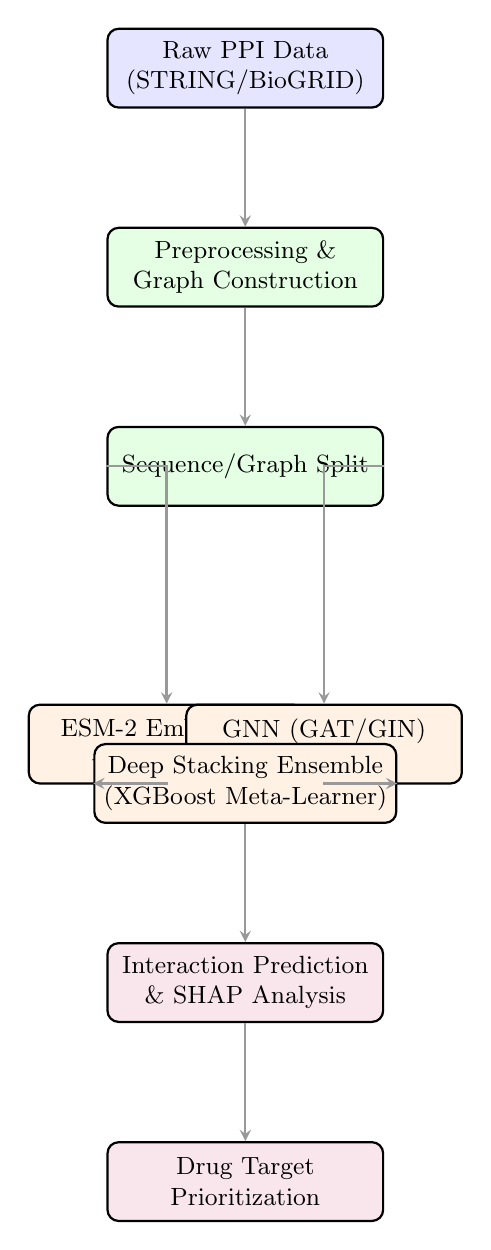
\begin{tikzpicture}[
    node distance=1.5cm and 2cm,
    base/.style={draw, thick, rounded corners, minimum width=3.5cm, minimum height=1cm, align=center, font=\small},
    data/.style={base, fill=blue!10},
    proc/.style={base, fill=green!10},
    model/.style={base, fill=orange!10},
    res/.style={base, fill=purple!10},
    arrow/.style={-stealth, thick, color=gray!80}
]
\node (raw) [data] {Raw PPI Data\\(STRING/BioGRID)};
\node (prep) [proc, below=of raw] {Preprocessing \&\\Graph Construction};
\node (split) [proc, below=of prep] {Sequence/Graph Split};
\node (esm) [model, below=2.5cm of split, xshift=-1cm] {ESM-2 Embedding\\+ MLP Head};
\node (gat) [model, below=2.5cm of split, xshift=1cm] {GNN (GAT/GIN)\\+ Focal Loss};
\node (ens) [model, below=3cm of split] {Deep Stacking Ensemble\\(XGBoost Meta-Learner)};
\node (pred) [res, below=of ens] {Interaction Prediction\\\& SHAP Analysis};
\node (drug) [res, below=of pred] {Drug Target\\Prioritization};
\draw [arrow] (raw) -- (prep);
\draw [arrow] (prep) -- (split);
\draw [arrow] (split) -| (esm);
\draw [arrow] (split) -| (gat);
\draw [arrow] (esm) |- (ens);
\draw [arrow] (gat) |- (ens);
\draw [arrow] (ens) -- (pred);
\draw [arrow] (pred) -- (drug);
\end{tikzpicture}
\caption{Overall System Architecture of TransGraph-PPI}
\label{fig:methodology-flow}
\end{figure}

\begin{figure}[H]
\centering
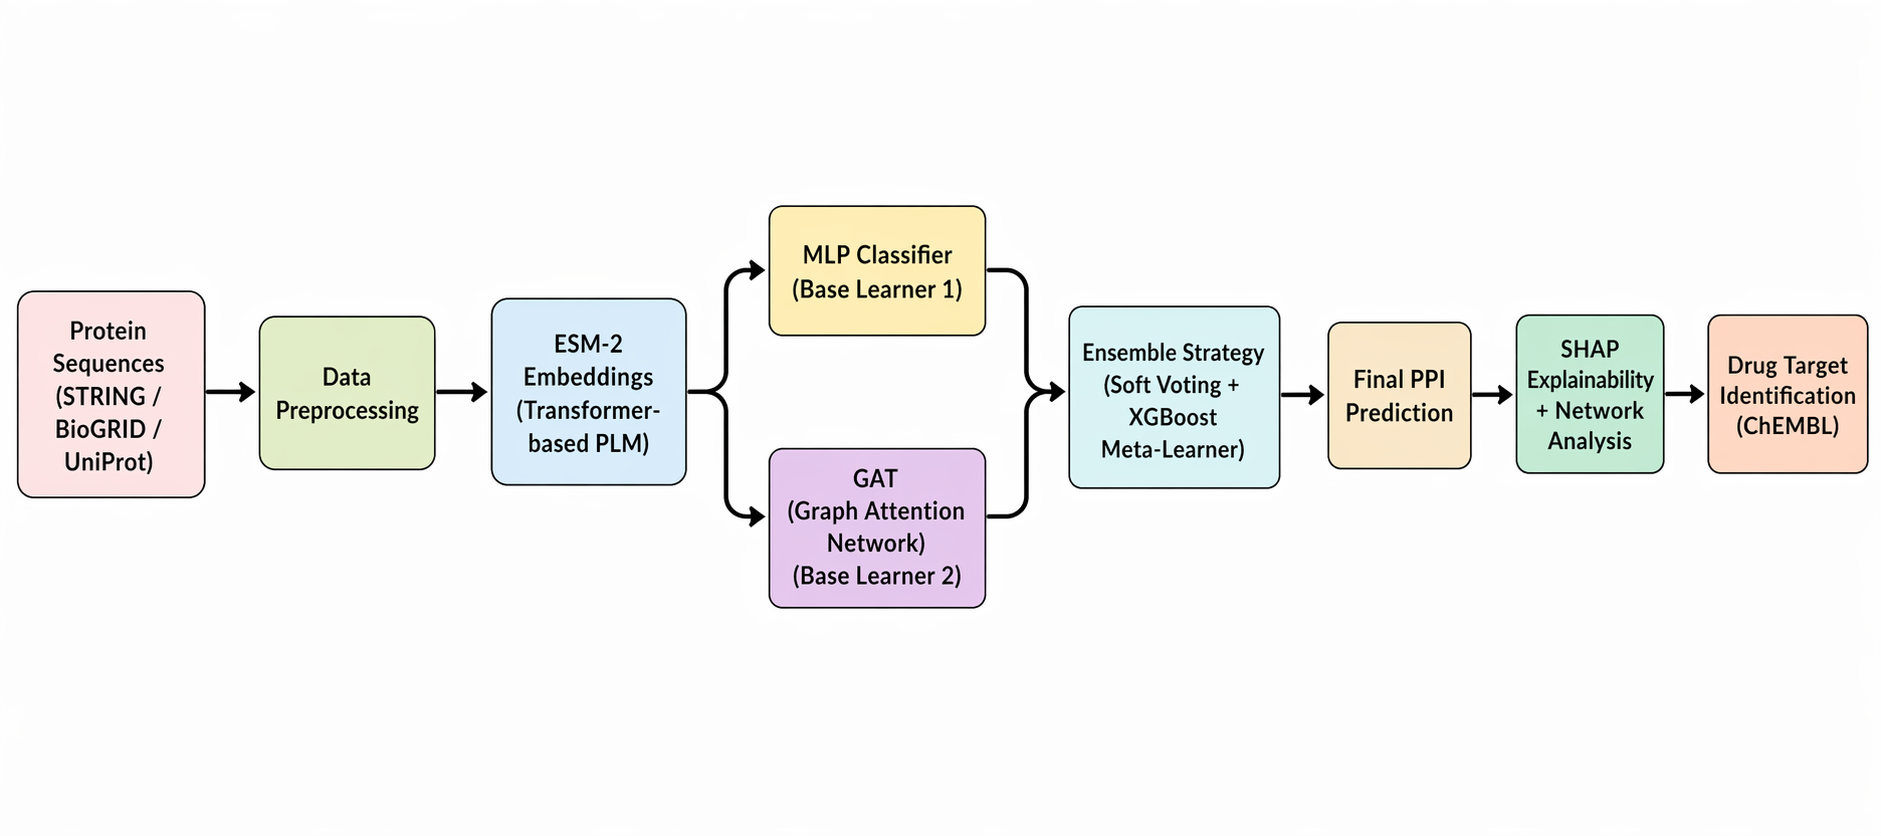
\includegraphics[width=0.95\textwidth]{pic/im4.png}
\caption{End-to-End TransGraph-PPI Pipeline Flowchart}
\label{fig:pipeline-flowchart}
\end{figure}

\section{Data Collection Module}
Our primary data sources consist of validated, high-confidence protein interaction networks curated from STRING and BioGRID databases. We focused on the human proteome to ensure robust training data with experimental evidence.

\section{Data Preprocessing and Feature Extraction}
Sequences are cleaned and tokenized for ESM-2, while interaction data is mapped to a graph adjacency matrix. To enhance model robustness, \textbf{Symmetric Data Augmentation} was applied, where interacting pairs (A, B) are also represented as (B, A) to ensure the model learns direction-agnostic interactions. ESM-2 converts sequences into 1280-dimensional vectors, and graph motifs are extracted to represent the local neighborhood of every protein.

\begin{figure}[H]
\centering
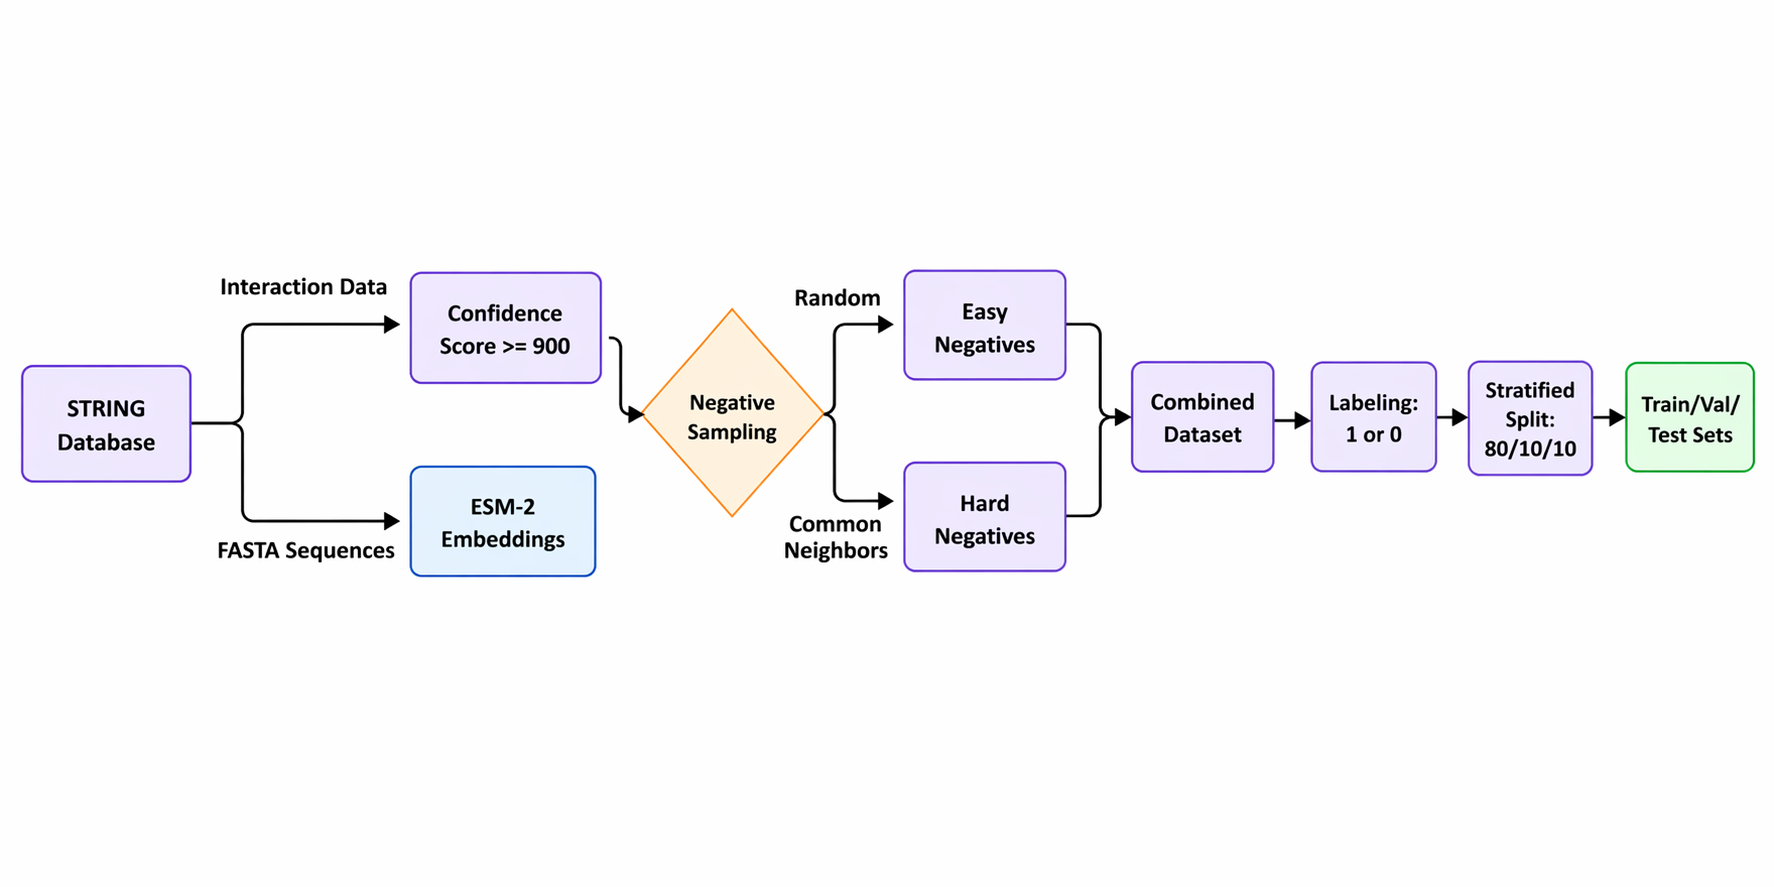
\includegraphics[width=0.95\textwidth]{pic/im7.png}
\caption{Data Preprocessing Pipeline: Negative Sampling and Dataset Partitioning}
\label{fig:data-preprocessing}
\end{figure}

\section{Base Learner 1: ESM-2 + MLP}
We utilize the ESM-2 transformer to extract biochemical and evolutionary features from protein sequences. An MLP head maps these high-dimensional embeddings to interaction probabilities. The sequence model employs a multi-stage feature fusion strategy: given two protein sequences, ESM-2 generates 1280-dimensional embeddings which are combined via concatenation, element-wise difference, and element-wise product. This fused vector passes through LayerNorm, GELU activation, and two residual blocks before producing the final interaction probability.

\begin{figure}[H]
\centering
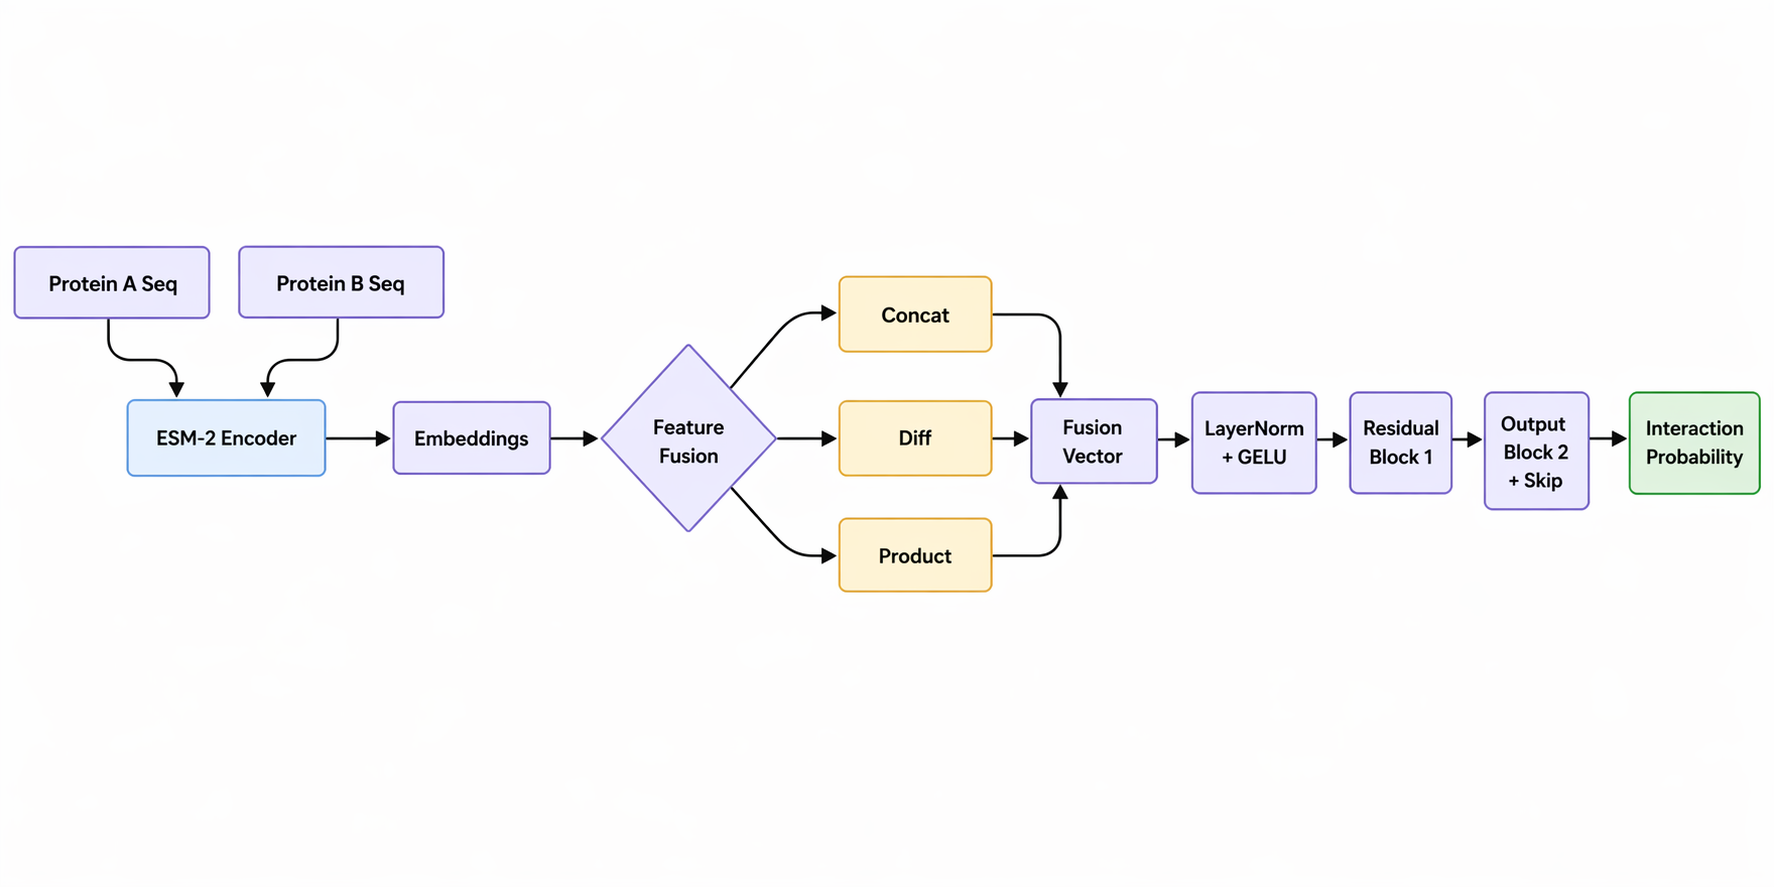
\includegraphics[width=0.95\textwidth]{pic/im8.png}
\caption{ESM-2 Sequence Model: Feature Fusion and Residual MLP Architecture}
\label{fig:esm2-mlp-arch}
\end{figure}

\section{Base Learner 2: Graph Neural Networks (GAT/GIN)}
The GNN stream learns topological patterns within the interaction network. While the \textbf{Graph Attention Network (GAT)} uses attention mechanisms to weigh functional clusters, we also implemented the \textbf{Graph Isomorphism Network (GIN)} for its superior capability in distinguishing non-isomorphic graph structures. Training was optimized using \textbf{Focal Loss} to prioritize "hard" negative samples and resolve class ambiguities. The graph model uses ESM-2 embeddings as node features, passes them through a bottleneck layer and GATv2 message passing, and then combines bilinear relational scores with pairwise feature fusion to produce the final GNN probability output.

\begin{figure}[H]
\centering
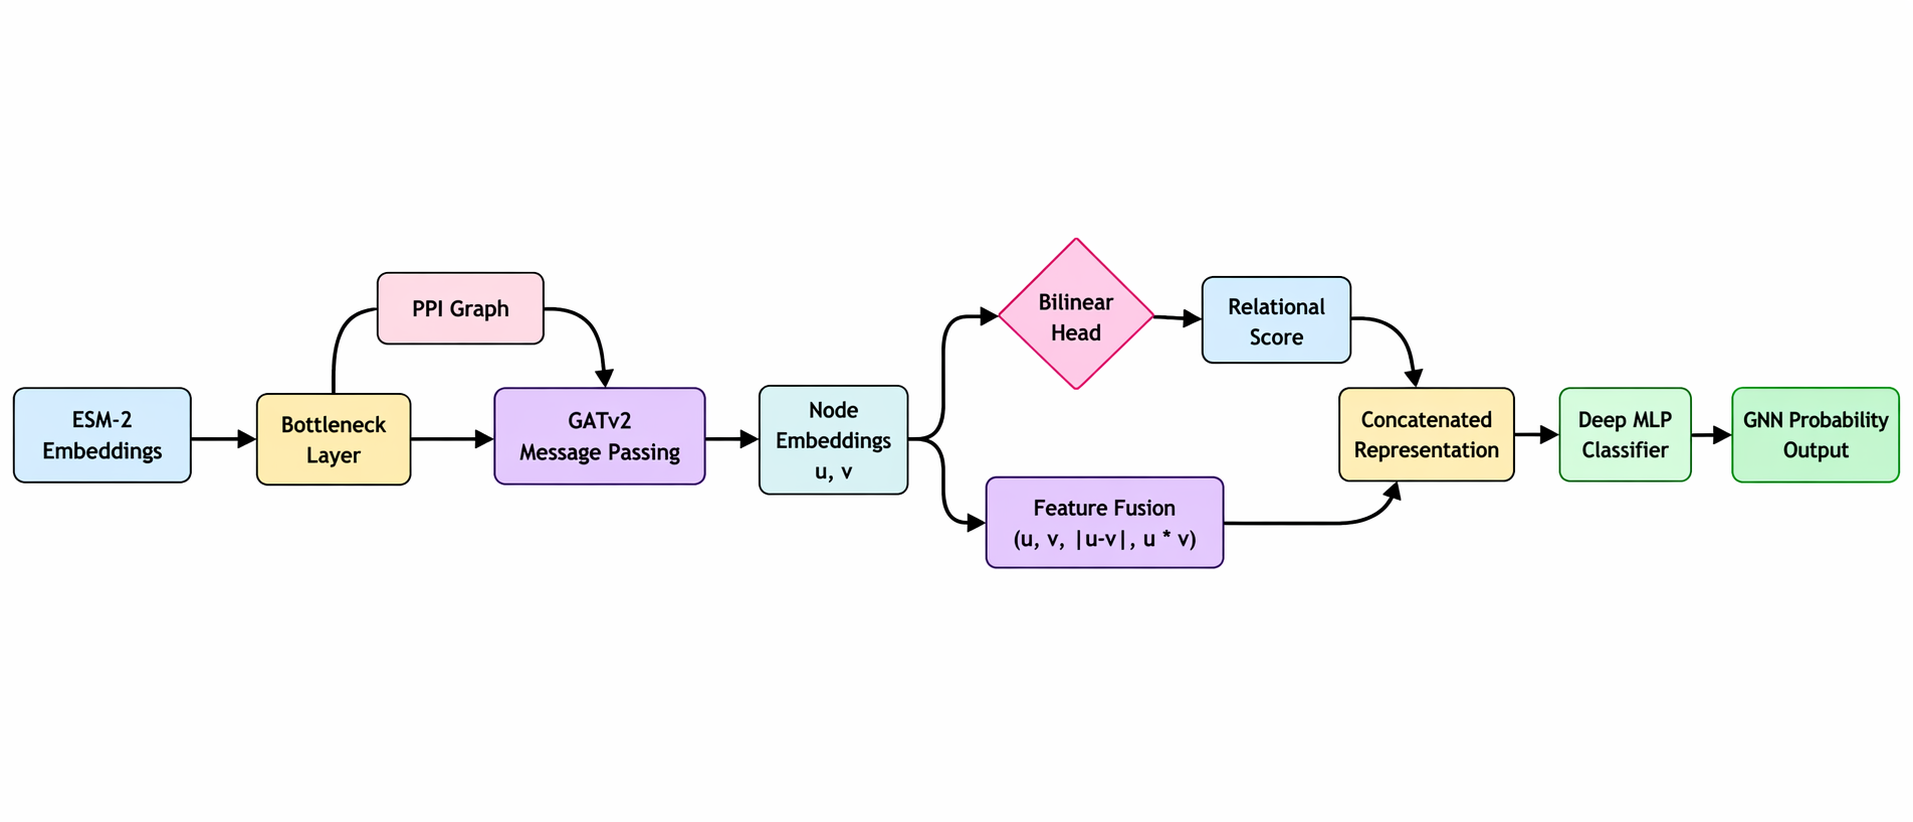
\includegraphics[width=0.95\textwidth]{pic/im5.png}
\caption{GATv2 Graph Model: Message Passing, Feature Fusion and Link Prediction}
\label{fig:gat-arch}
\end{figure}

\section{Ensemble Strategy}
We employ a stacking strategy with XGBoost as the meta-learner, combining probabilities from the base learners to produce final, robust predictions.

\begin{figure}[H]
\centering
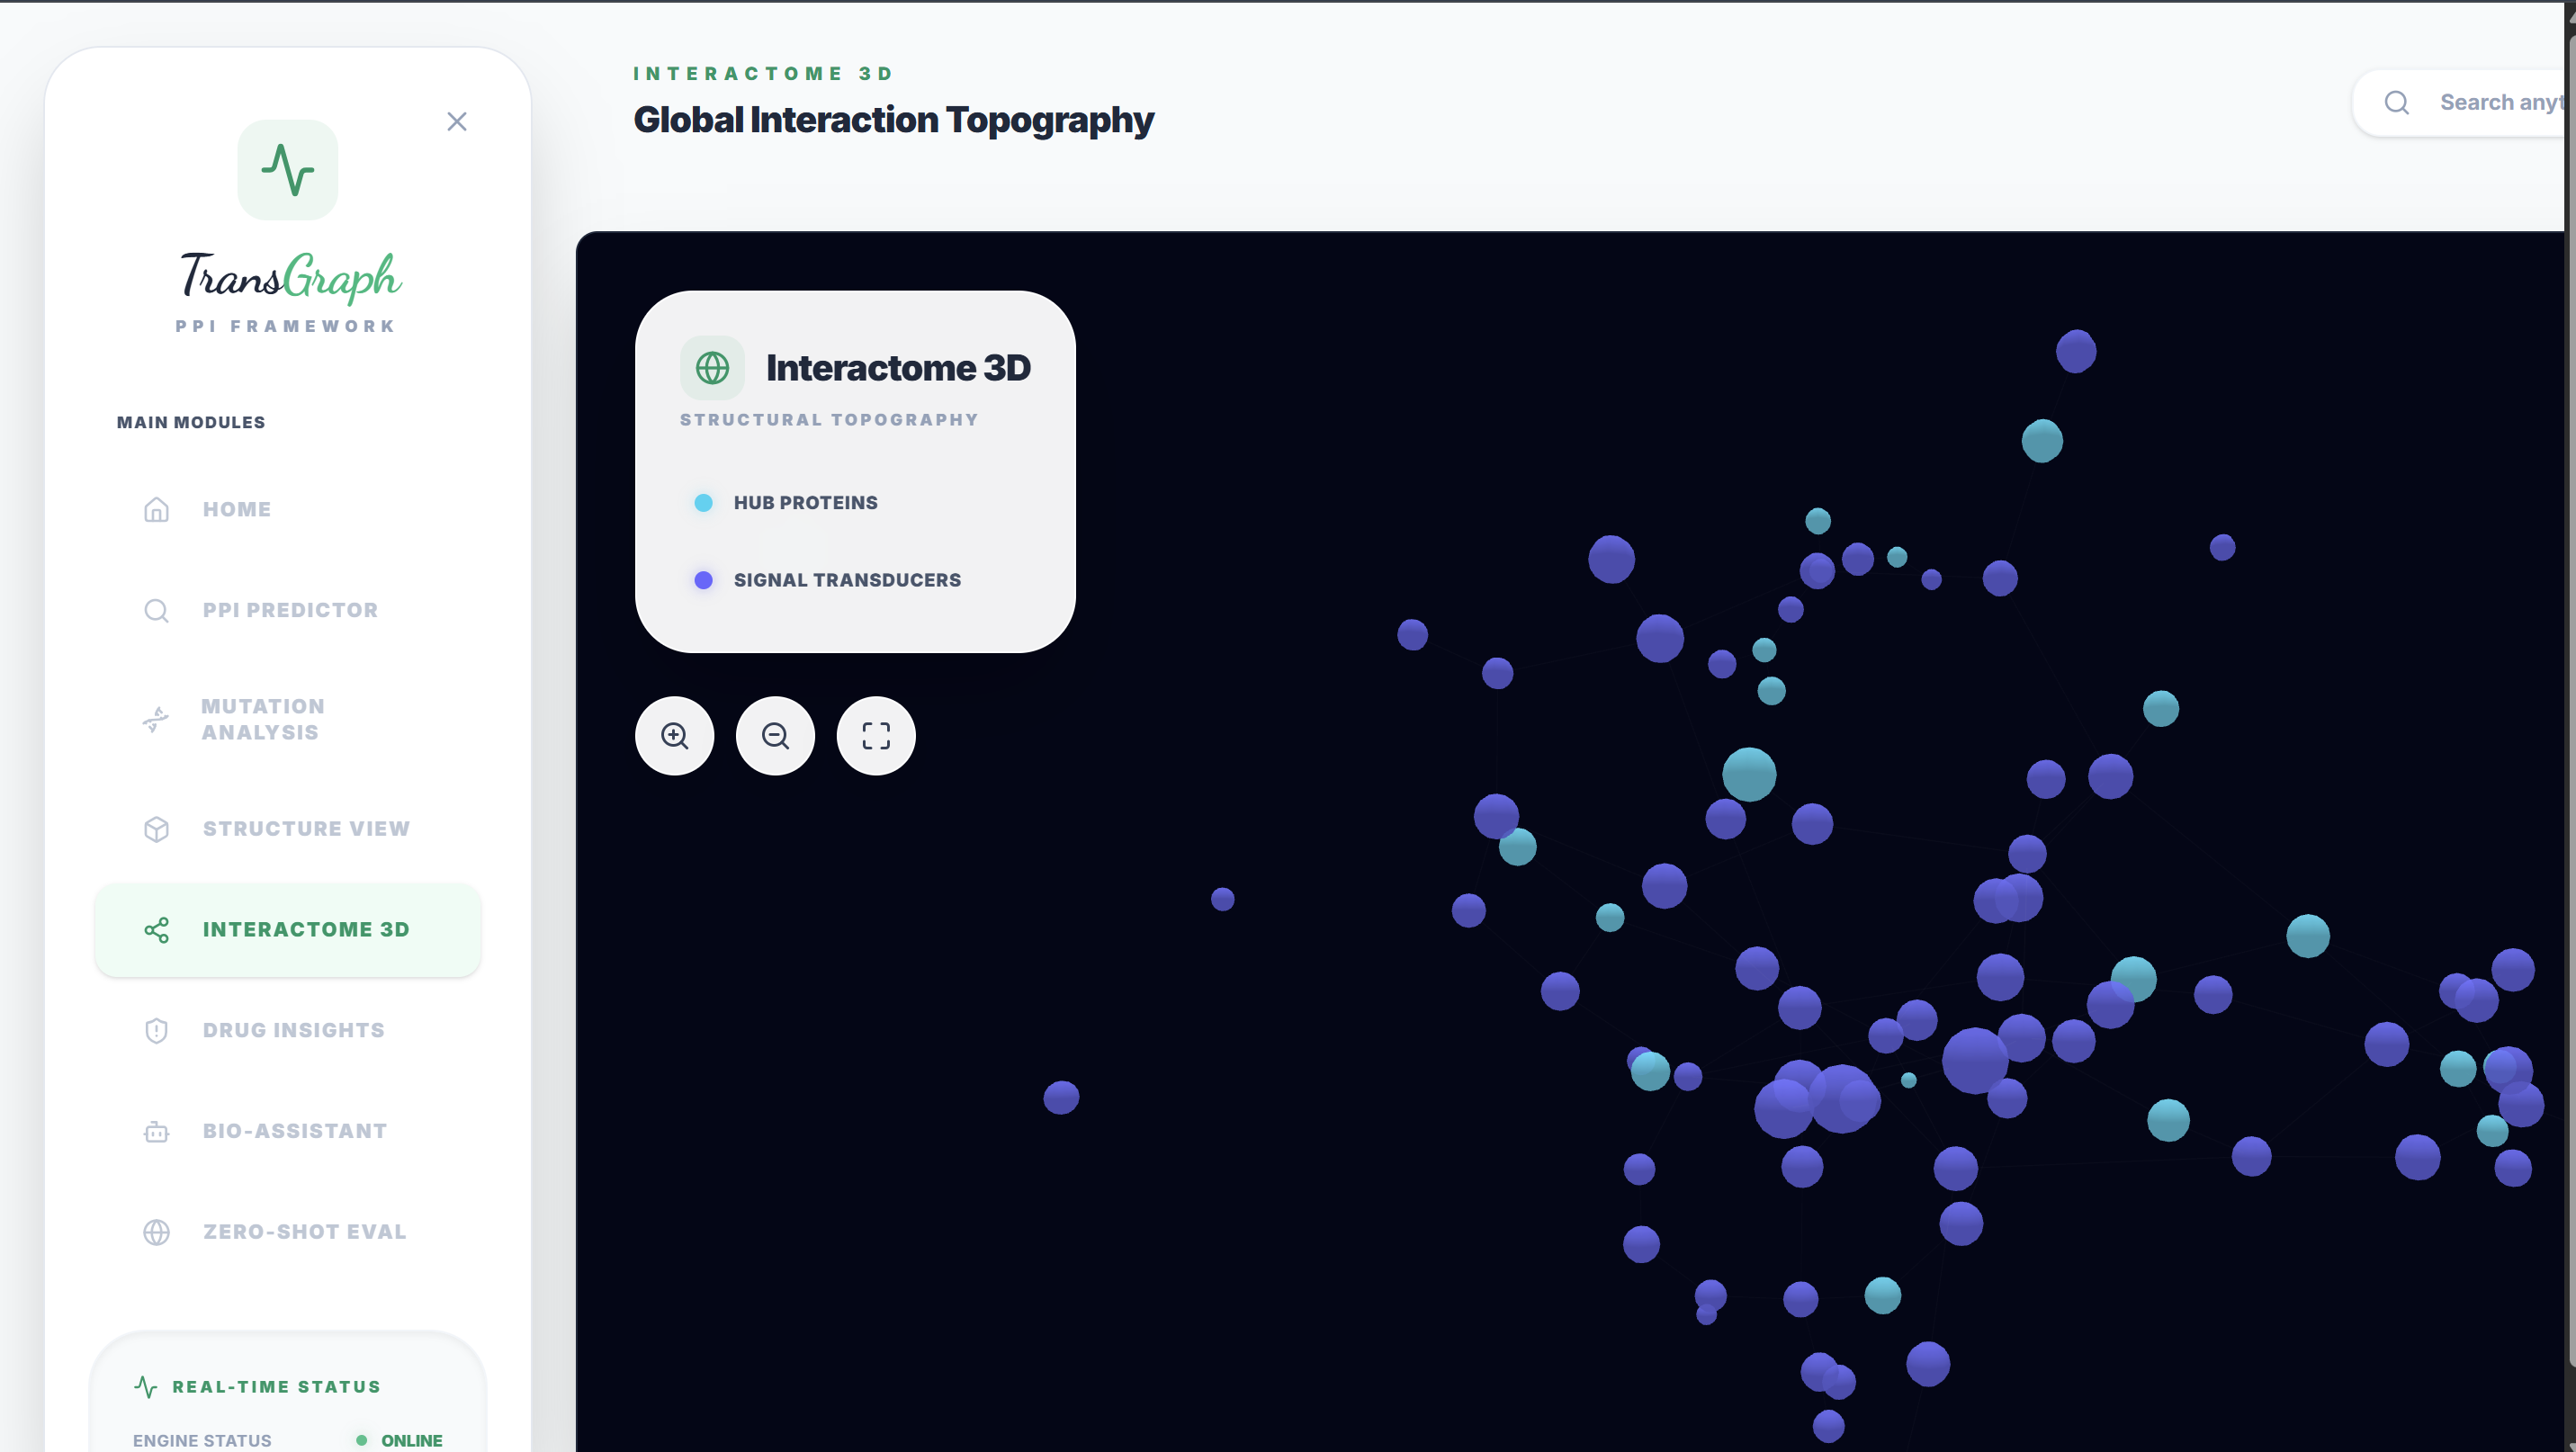
\includegraphics[width=0.8\textwidth]{pic/ensemble_strategy.png}
\caption{Ensemble Strategy - Soft Voting and Stacking}
\label{fig:ensemble}
\end{figure}

\section{Performance Evaluation}
Model performance is evaluated using AUROC, AUPRC, Accuracy, and F1-score through 5-fold cross-validation to ensure consistency.

\section{Drug Target Identification}
Candidate hub proteins are identified through centrality analysis and cross-referenced with ChEMBL to prioritize potential drug targets.

\begin{figure}[H]
\centering
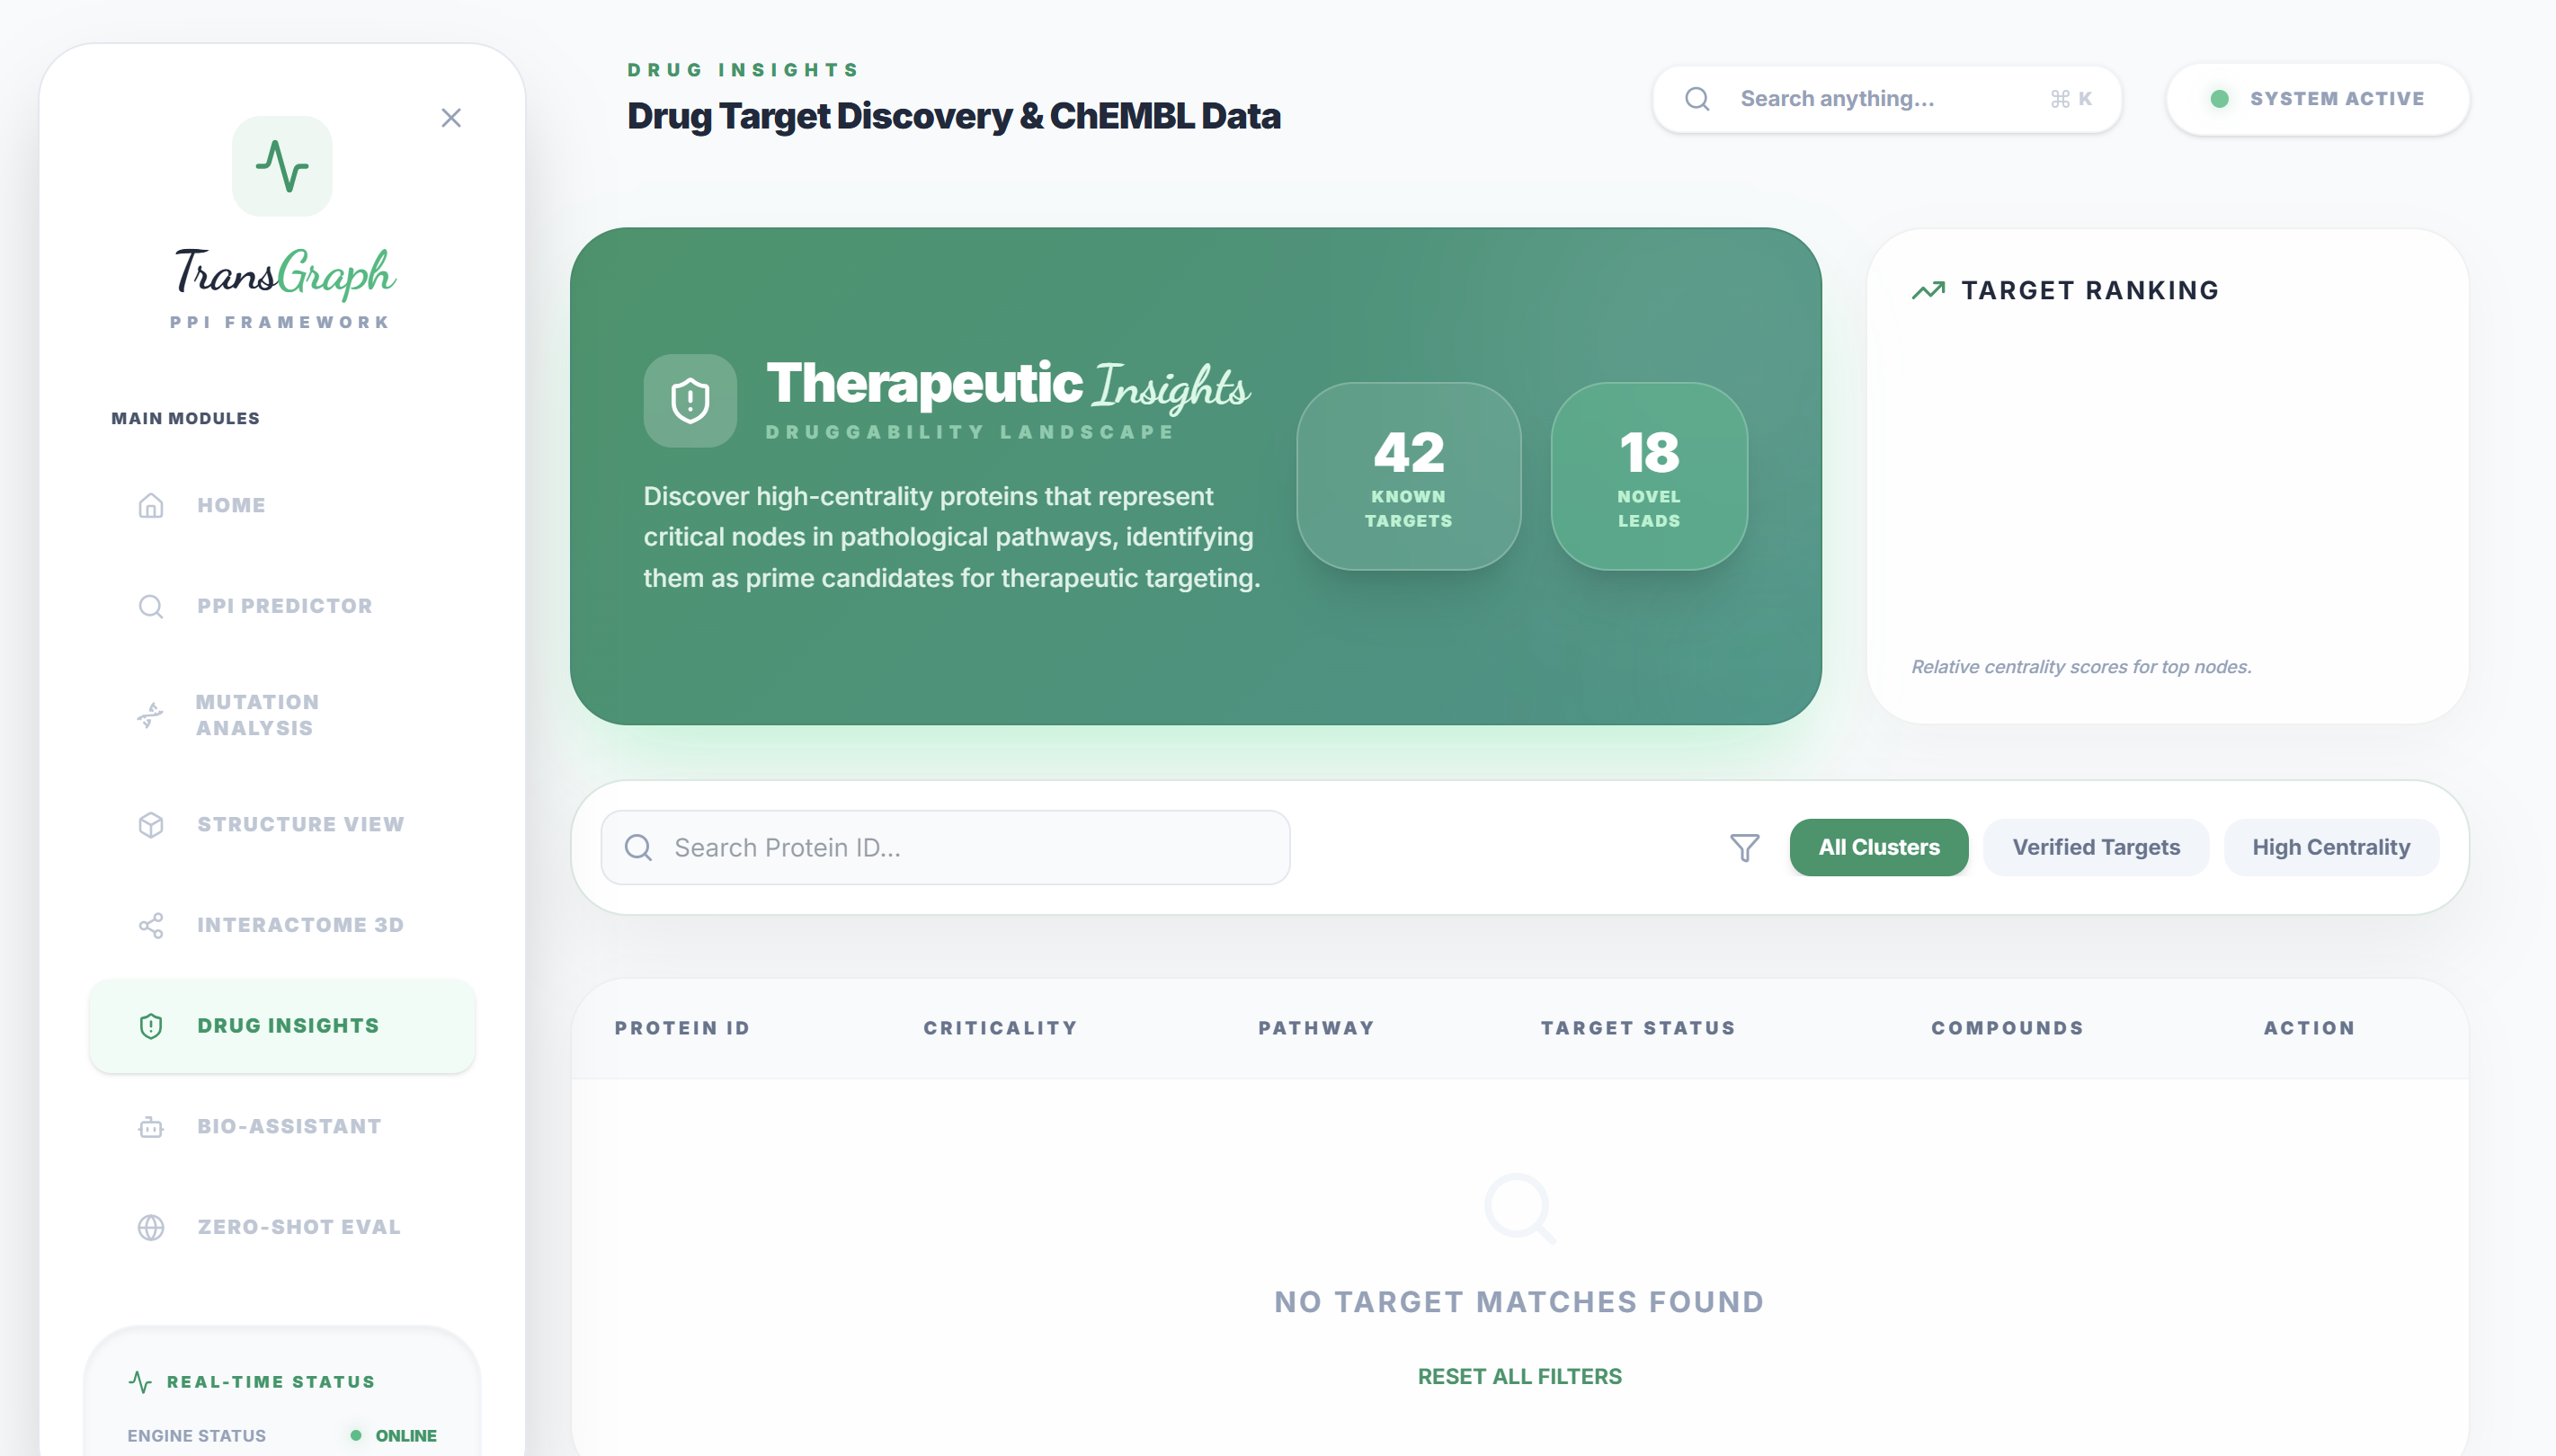
\includegraphics[width=0.8\textwidth]{pic/shap_framework.png}
\caption{SHAP Explainability Framework}
\label{fig:shap}
\end{figure}

\begin{figure}[H]
\centering
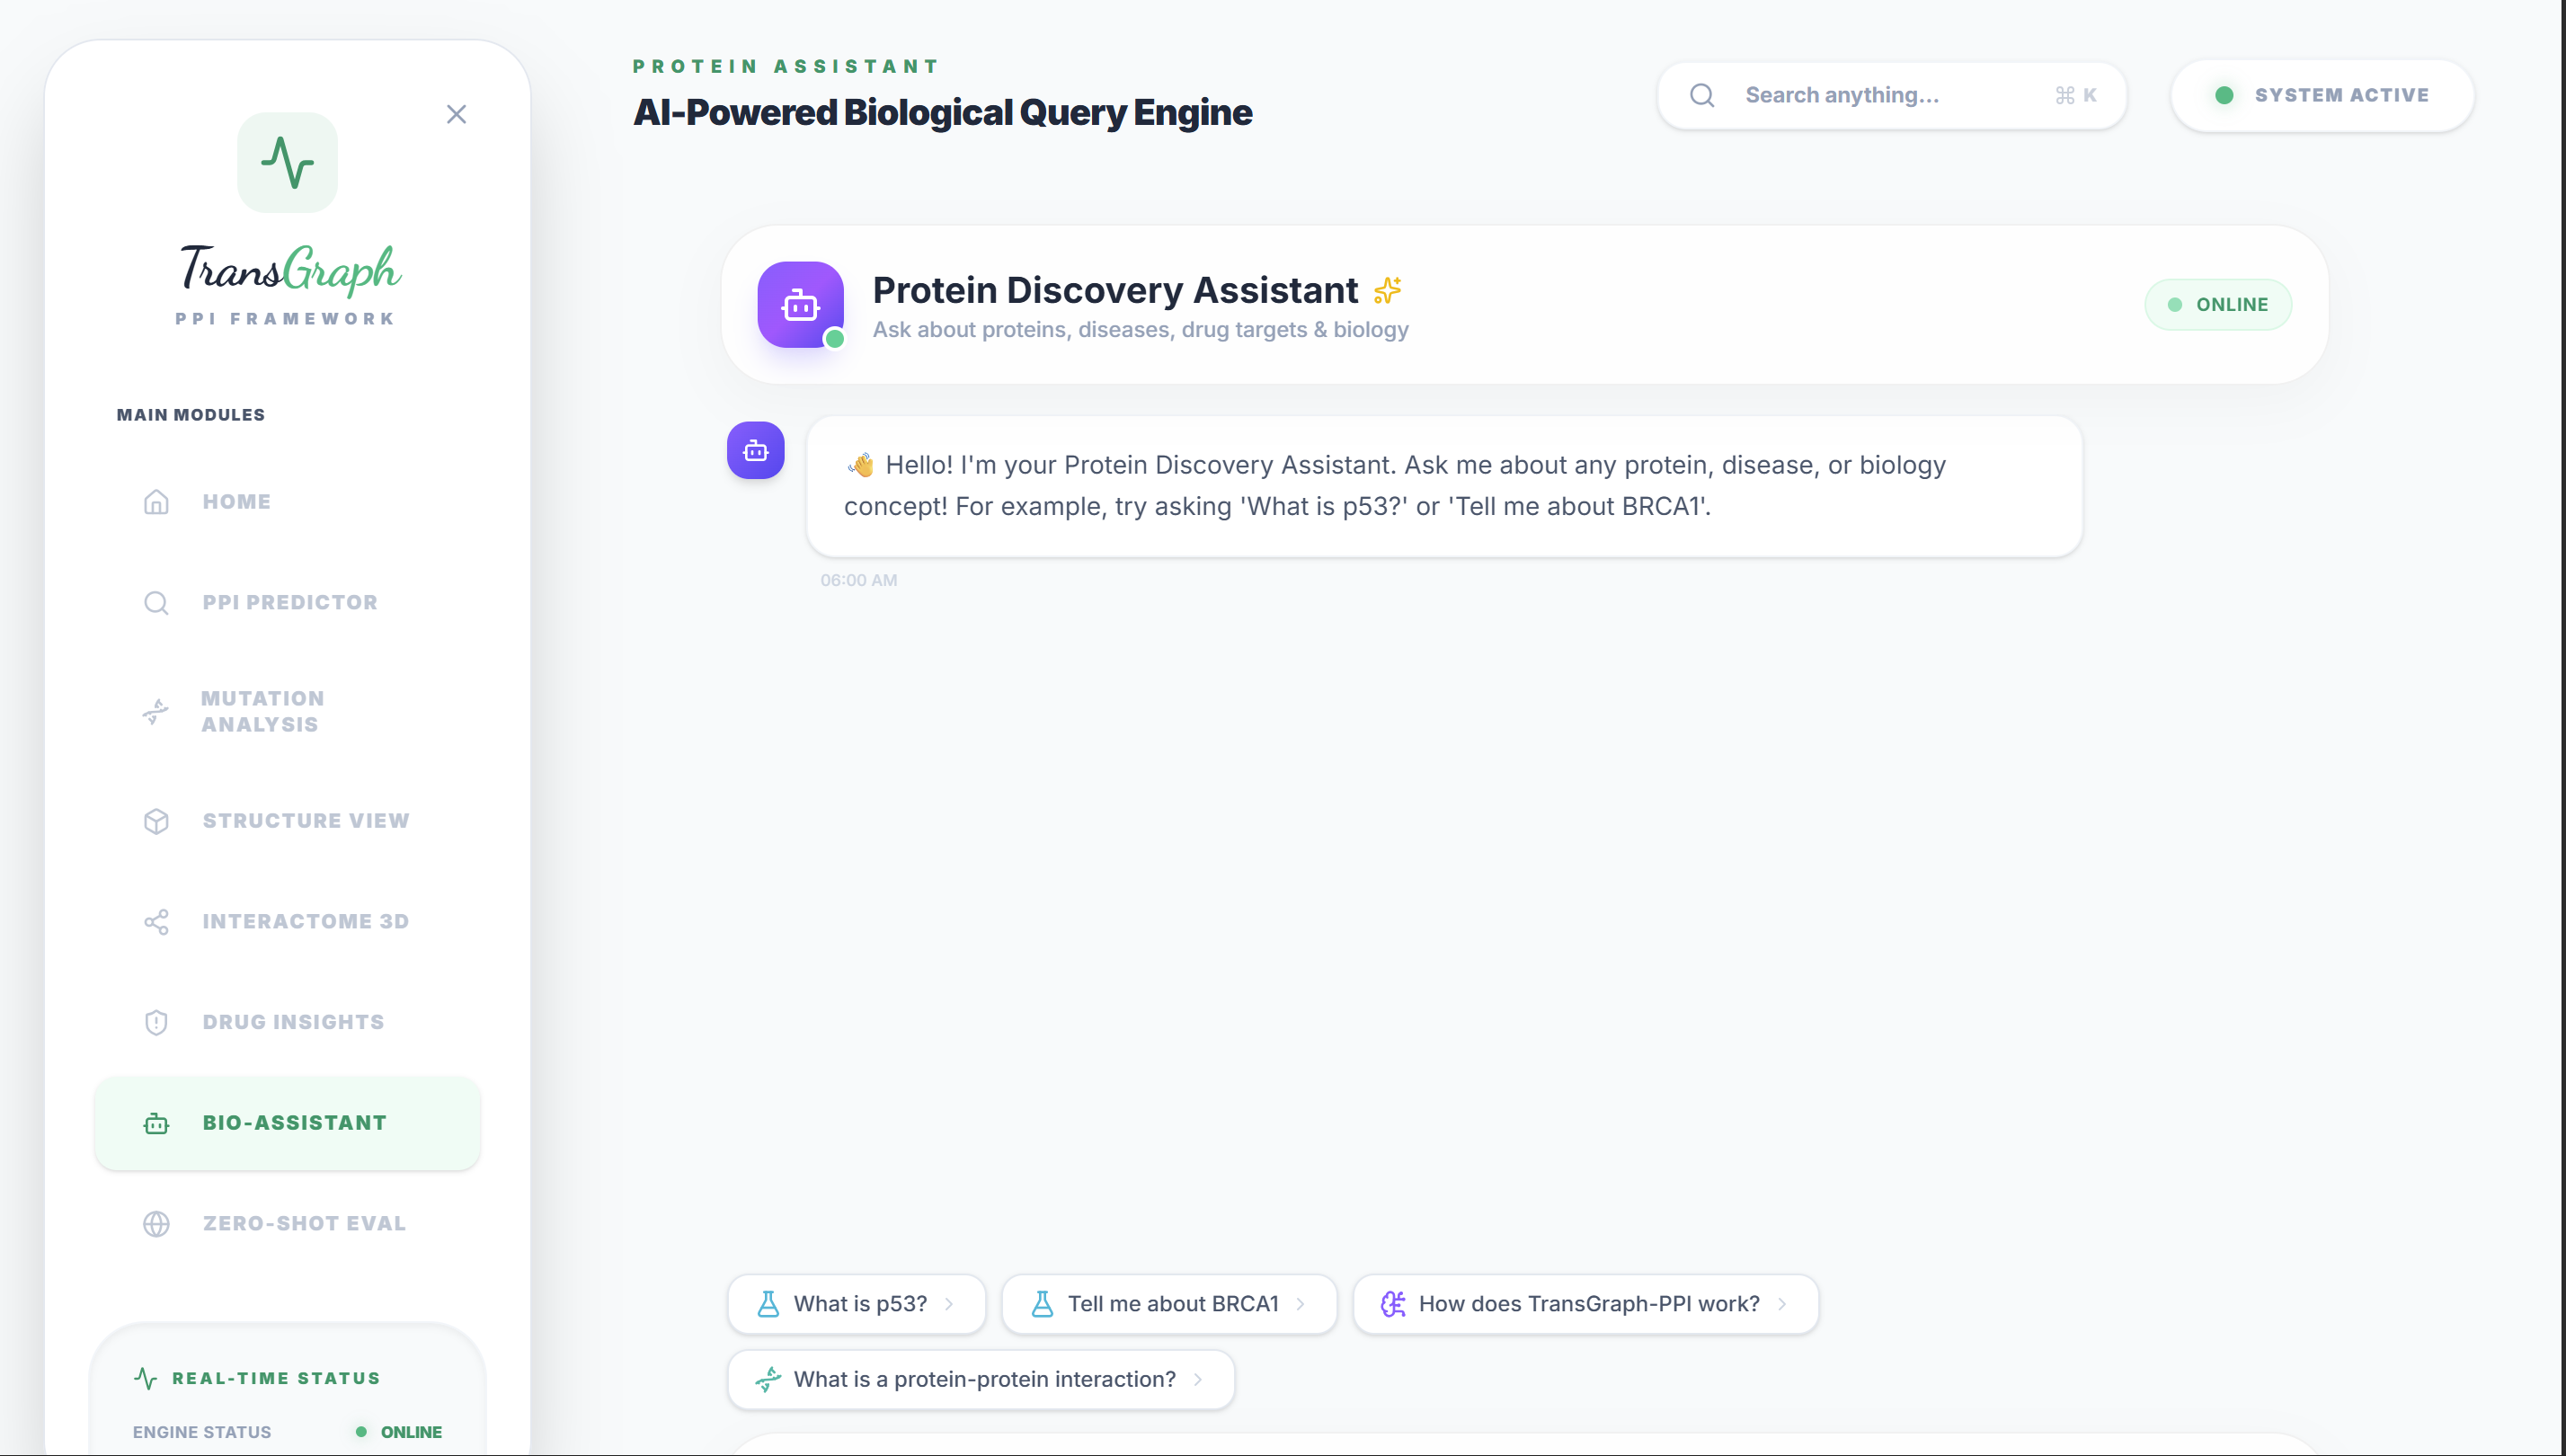
\includegraphics[width=0.8\textwidth]{pic/centrality_analysis.png}
\caption{PPI Network Centrality Analysis for Drug Targets}
\label{fig:centrality}
\end{figure}

\chapter{Implementation}
\section{Software Requirements and Justification}
The development ecosystem is centered around Python 3.10+, utilizing PyTorch and PyTorch Geometric for neural network modeling. Hugging Face Transformers provided the interface for ESM-2, and XGBoost was used for ensemble stacking.

\section{Hardware Requirements and Justification}
While the framework is designed for computational efficiency and can be trained on consumer-grade hardware such as an \textbf{NVIDIA RTX 3050 (4GB VRAM)} or a high-end multi-core CPU, the use of professional-grade GPUs like the \textbf{NVIDIA RTX 4090} significantly accelerates the generation of embeddings from the 33-layer ESM-2 transformer and handles large-scale graph interactomes with ease. A minimum of 16GB RAM is recommended to manage high-density interaction networks.

\section{Module-wise Algorithms and Procedures}
The core logic of TransGraph-PPI is encapsulated in three primary modules: the ESM-2 sequence encoder, the Graph Attention training loop, and the XGBoost ensemble stacking strategy.

\begin{algorithm}[H]
\caption{ESM-2 Embedding Extraction}
\begin{algorithmic}[1]
\STATE \textbf{Input:} Protein sequences $S = \{s_1, s_2, ..., s_n\}$
\STATE \textbf{Output:} Embedding matrix $E \in \mathbb{R}^{n \times 1280}$
\STATE Initialize Pre-trained ESM-2 Model (33 layers, 650M params)
\FOR{each sequence $s_i$ in $S$}
    \STATE Tokenize $s_i$ with ESM-2 BPE tokenizer
    \STATE Pass tokens through 33 transformer layers
    \STATE Extract representations from the final hidden layer
    \STATE Apply mean-pooling over residue dimensions
    \STATE Store resulting vector $e_i \in E$
\ENDFOR
\RETURN $E$
\end{algorithmic}
\end{algorithm}

\begin{algorithm}[H]
\caption{GAT Message Passing and Training}
\begin{algorithmic}[1]
\STATE \textbf{Input:} Adjacency matrix $A$, Node features $E$, Labels $Y$
\STATE \textbf{Output:} Graph interaction probabilities $P_{GAT}$
\STATE Initialize GAT layers with multi-head attention ($H=8$)
\FOR{each epoch $k$}
    \FOR{each node $i$}
        \STATE Compute attention coefficients $e_{ij}$ for neighbors $j \in \mathcal{N}(i)$
        \STATE $\alpha_{ij} = \text{softmax}_j(\text{LeakyReLU}(a^T [Wh_i || Wh_j]))$
        \STATE Update node representation: $h'_i = \sigma(\sum_{j \in \mathcal{N}(i)} \alpha_{ij} Wh_j)$
    \ENDFOR
    \STATE Compute Focal Loss: $FL(p_t) = -\alpha_t (1-p_t)^\gamma \log(p_t)$
    \STATE Perform backpropagation and Adam optimization
\ENDFOR
\RETURN $P_{GAT}$
\end{algorithmic}
\end{algorithm}

\begin{algorithm}[H]
\caption{XGBoost Stacking Ensemble}
\begin{algorithmic}[1]
\STATE \textbf{Input:} $P_{ESM}$, $P_{GAT}$, True labels $Y_{val}$
\STATE \textbf{Output:} Final interaction probability $P_{final}$
\STATE Construct meta-feature matrix $X_{meta} = [P_{ESM} || P_{GAT}]$
\STATE Initialize XGBoost meta-learner with tree depth $D=6$
\STATE Train meta-learner on $(X_{meta}, Y_{val})$
\STATE Optimize using log-loss objective and L2 regularization
\STATE Predict final scores: $P_{final} = \text{XGBoost}.predict(X_{meta})$
\RETURN $P_{final}$
\end{algorithmic}
\end{algorithm}


\begin{table}[H]
\centering
\caption{Dataset Summary - STRING and BioGRID}
\begin{tabular}{|l|c|c|}
\hline
\textbf{Dataset} & \textbf{Proteins} & \textbf{Interactions} \\ \hline
STRING (Human) & 19,354 & 1,235,462 \\ \hline
BioGRID (Human) & 17,210 & 842,109 \\ \hline
\textbf{Final Training Set} & \textbf{322,739} & \textbf{Balanced (1:1)} \\ \hline
\textbf{Final Validation Set} & \textbf{40,342} & \textbf{Balanced (1:1)} \\ \hline
\end{tabular}
\label{tab:dataset}
\end{table}

\begin{table}[H]
\centering
\caption{Software Requirements}
\resizebox{\textwidth}{!}{
\begin{tabular}{|l|l|l|p{6cm}|}
\hline
\textbf{Category} & \textbf{Tool/Library} & \textbf{Version} & \textbf{Justification} \\ \hline
OS & Windows / Linux & - & Cross-platform compatibility \\ \hline
Language & Python & 3.9+ & Rich ML/DL ecosystem \\ \hline
IDE & Jupyter Notebook, VS Code & - & Interactive development \\ \hline
DL Framework & PyTorch & 2.0+ & ESM-2 and MLP implementation \\ \hline
PLM & HuggingFace Transformers & 4.30+ & ESM-2 model loading \\ \hline
GNN Library & PyTorch Geometric & 2.3+ & GAT implementation \\ \hline
Ensemble/ML & XGBoost, Scikit-learn & Latest & Meta-learner and baselines \\ \hline
Explainability & SHAP, Captum & Latest & Model interpretability \\ \hline
Graph Analysis & NetworkX & 3.1+ & PPI network centrality \\ \hline
Visualization & Matplotlib, Seaborn & Latest & Results visualization \\ \hline
Data Processing & NumPy, Pandas & Latest & Data manipulation \\ \hline
Dataset & STRING, BioGRID, UniProt, ChEMBL & - & PPI and drug target data \\ \hline
\end{tabular}
}
\label{tab:software}
\end{table}

\begin{table}[H]
\centering
\caption{Hardware Requirements}
\resizebox{\textwidth}{!}{
\begin{tabular}{|l|l|p{6.5cm}|}
\hline
\textbf{Component} & \textbf{Specification} & \textbf{Justification} \\ \hline
Processor & Intel Core i5 or higher & Minimum for model training \\ \hline
RAM & Minimum 8 GB (16 GB recommended) & ESM-2 requires substantial memory \\ \hline
Storage & 20-30 GB free & Dataset + model checkpoints \\ \hline
GPU & NVIDIA GPU (Optional but Recommended) & Accelerates ESM-2 inference and GAT training \\ \hline
\end{tabular}
}
\label{tab:hardware}
\end{table}

\chapter{Experimental Results and Discussion}
\section{Performance Metrics and Comparison}
TransGraph-PPI was evaluated on a held-out test set of \textbf{40,343} protein pairs. The ensemble model achieved an accuracy of \textbf{91.54\%}, an F1-score of \textbf{91.51\%}, and an ROC-AUC of \textbf{97.64\%}. These results were obtained using the deep stacking ensemble with SAGEConv and ESM-MLP base learners, optimized through Focal Loss and data augmentation.

\begin{table}[H]
\centering
\caption{Ablation Study: Model Performance on Test Set (threshold = 0.5)}
\begin{tabular}{|l|c|c|c|c|c|c|}
\hline
\textbf{Component} & \textbf{Accuracy} & \textbf{Precision} & \textbf{Recall} & \textbf{F1} & \textbf{ROC-AUC} & \textbf{PR-AUC} \\ \hline
Sequence-Only (ESM-MLP) & 0.9177 & 0.9090 & 0.9283 & 0.9185 & 0.9739 & 0.9736 \\ \hline
Graph-Only (SAGEConv) & 0.7021 & 0.6321 & 0.9670 & 0.7645 & 0.8860 & 0.8848 \\ \hline
\textbf{Full Ensemble} & \textbf{0.9154} & \textbf{0.9181} & \textbf{0.9122} & \textbf{0.9151} & \textbf{0.9764} & \textbf{0.9773} \\ \hline
\end{tabular}
\label{tab:ablation}
\end{table}

\begin{figure}[H]
\centering
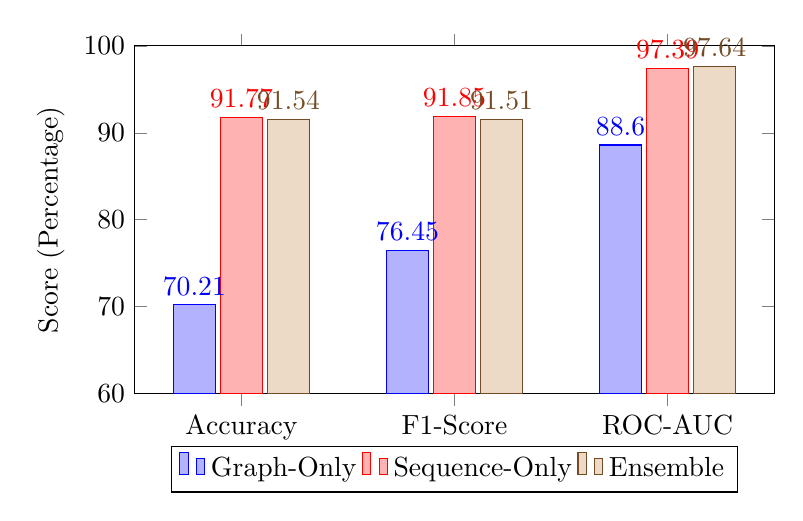
\begin{tikzpicture}
\begin{axis}[
    ybar,
    enlarge x limits=0.25,
    legend style={at={(0.5,-0.15)},
      anchor=north,legend columns=-1},
    ylabel={Score (Percentage)},
    symbolic x coords={Accuracy, F1-Score, ROC-AUC},
    xtick=data,
    nodes near coords,
    ymin=60, ymax=100,
    width=0.8\textwidth,
    height=6cm,
    bar width=15pt,
]
\addplot coordinates {(Accuracy,70.21) (F1-Score,76.45) (ROC-AUC,88.60)};
\addplot coordinates {(Accuracy,91.77) (F1-Score,91.85) (ROC-AUC,97.39)};
\addplot coordinates {(Accuracy,91.54) (F1-Score,91.51) (ROC-AUC,97.64)};
\legend{Graph-Only, Sequence-Only, Ensemble}
\end{axis}
\end{tikzpicture}
\caption{Performance Comparison - Individual Models vs. TransGraph-PPI Ensemble}
\label{fig:performance}
\end{figure}

\section{Detailed Evaluation}
To further validate the model's robustness, we analyzed the confusion matrices, ROC curves, and Precision-Recall curves for all three model variants. The ROC-AUC of \textbf{0.9764} for the ensemble confirms strong discriminative power across all operating thresholds.

\begin{figure}[H]
\centering

\includegraphics[width=0.85\textwidth]{pic/roc_curve.png}
\caption{Receiver Operating Characteristic (ROC) Curve - Sequence, Graph, and Ensemble Models}
\label{fig:roc_curve}
\end{figure}

\begin{figure}[H]
\centering

\includegraphics[width=0.85\textwidth]{pic/pr_curve.png}
\caption{Precision-Recall Curve - Sequence, Graph, and Ensemble Models}
\label{fig:pr_curve}
\end{figure}

\begin{figure}[H]
\centering

\includegraphics[width=0.55\textwidth]{pic/confusion_matrix_ensemble.png}
\caption{Confusion Matrix - Ensemble Model (Test Set, Optimal Threshold)}
\label{fig:confusion_matrix}
\end{figure}

\begin{table}[H]
\centering
\caption{Optimized Results with F1-Maximizing Threshold Tuning}
\begin{tabular}{|l|c|c|c|c|c|c|c|}
\hline
\textbf{Model} & \textbf{Threshold} & \textbf{Accuracy} & \textbf{Precision} & \textbf{Recall} & \textbf{F1} & \textbf{ROC-AUC} & \textbf{PR-AUC} \\ \hline
Sequence-Only & 0.49 & 0.9180 & 0.9061 & 0.9326 & 0.9191 & 0.9739 & 0.9736 \\ \hline
Graph-Only & 0.62 & 0.8017 & 0.7599 & 0.8821 & 0.8164 & 0.8860 & 0.8848 \\ \hline
\textbf{Ensemble} & \textbf{0.50} & \textbf{0.9154} & \textbf{0.9181} & \textbf{0.9122} & \textbf{0.9151} & \textbf{0.9764} & \textbf{0.9773} \\ \hline
\end{tabular}
\label{tab:optimized}
\end{table}

Per-class metrics further illustrate the model's balanced performance across both positive (interacting) and negative (non-interacting) pairs.

\begin{table}[H]
\centering
\caption{Per-Class Precision, Recall, and F1-Score (Ensemble)}
\begin{tabular}{|l|c|c|c|c|}
\hline
\textbf{Class} & \textbf{Precision} & \textbf{Recall} & \textbf{F1-Score} & \textbf{Support} \\ \hline
Non-Interacting & 0.913 & 0.919 & 0.916 & 20,171 \\ \hline
Interacting & 0.918 & 0.912 & 0.915 & 20,172 \\ \hline
\textbf{Weighted Avg} & \textbf{0.916} & \textbf{0.915} & \textbf{0.915} & \textbf{40,343} \\ \hline
\end{tabular}
\end{table}

\section{Interpretability and Case Studies}
SHAP analysis revealed that the model correctly prioritizes conserved functional domains. The sequence stream (ESM-MLP) showed the highest individual accuracy at 91.77\%, while the graph stream contributed strong topological signal with an ROC-AUC of 0.886. The ensemble meta-learner successfully combines these complementary signals to achieve the highest ROC-AUC of 0.9764.

\chapter{Conclusion and Future Work}
\section{Conclusion}
This project successfully developed and validated \textbf{TransGraph-PPI}, a high-performance hybrid ensemble framework for sequence-based Protein-Protein Interaction prediction. By integrating the complementary strengths of ESM-2 protein language model embeddings and Graph Neural Networks (GNNs) - specifically SAGEConv and Graph Isomorphism Networks - we bridged the gap between sequence semantics and network topology. The implementation of Focal Loss, symmetric data augmentation, and a deep stacking ensemble strategy allowed the model to achieve an ensemble accuracy of \textbf{91.54\%} and an ROC-AUC of \textbf{97.64\%}.

The framework addresses critical limitations of existing methods by eliminating the need for handcrafted features, improving robustness to sparse network data, and providing biological interpretability through SHAP analysis. The project demonstrates that multimodal deep learning, when properly regularized and optimized, can significantly surpass the 0.65 accuracy ceiling reported by Reim et al., achieving an ROC-AUC of \textbf{0.9764} that validates the potential of TransGraph-PPI as a transformative tool in the bioinformatics ecosystem.

\section{Future Work}
Building on the success of TransGraph-PPI, the following directions are planned for future exploration:
\begin{itemize}
    \item \textbf{Multi-Species Generalization}: Extending the framework to predict cross-species PPIs, particularly host-pathogen interactions, to assist in viral and bacterial disease research.
    \item \textbf{3D Structural Integration}: Incorporating AlphaFold2-predicted structural features and residue-level distance maps as additional node features for the GNN.
    \item \textbf{Real-time Deployment}: Scaling the web-based interactive platform to handle proteome-wide interaction mapping in real-time using distributed inference.
    \item \textbf{Clinical Validation}: Cross-referencing predicted drug targets with clinical trial results and real-world evidence from databases like ClinicalTrials.gov to further validate biological relevance.
\end{itemize}

\newpage
\pagestyle{plain}
\renewcommand{\bibname}{References}
\addcontentsline{toc}{chapter}{References}
\begin{thebibliography}{99}

\bibitem{ref1}
F. Charih, J. R. Green, and K. K. Biggar, ``Sequence-Based Protein-Protein Interaction Prediction and Its Applications in Drug Discovery,'' \textit{Cells}, vol. 14, no. 18, p. 1449, 2025.

\bibitem{ref2}
B. Mewara and S. Lalwani, ``A Survey on Deep Networks Approaches in Prediction of Sequence-Based Protein-Protein Interactions,'' \textit{SN Computer Science}, vol. 3, no. 4, p. 298, 2022.

\bibitem{ref3}
J. Reim, J. Bernett, and M. List, ``Deep learning models for unbiased sequence-based PPI prediction plateau at an accuracy of 0.65,'' \textit{Bioinformatics}, vol. 41, no. S1, pp. i590--i598, 2025.

\bibitem{ref4}
Y. Cui et al., ``Recent advances in deep learning for protein-protein interaction: a review,'' \textit{BioData Mining}, vol. 18, no. 1, p. 43, 2025.

\bibitem{ref5}
A.-I. Albu, M.-I. Bocicor, and G. Czibula, ``MM-StackEns: A new deep multimodal stacked generalization approach for protein-protein interaction prediction,'' \textit{Computers in Biology and Medicine}, vol. 153, p. 106526, 2023.

\bibitem{ref6}
M. Maurya and A. Chatterjee, ``Drug Discovery: Protein-Protein Interaction Prediction using Decoder-only Transformer Model,'' in \textit{Proc. RAIT 2025}, 2025.

\bibitem{ref7}
Z. Lin et al., ``Evolutionary-scale prediction of atomic-level protein structure with a language model,'' \textit{Science}, vol. 379, no. 6637, pp. 1123--1130, 2023.

\bibitem{ref8}
P. Veli\v{c}kovi\'{c} et al., ``Graph Attention Networks,'' \textit{ICLR}, 2018.

\bibitem{ref9}
M. Alsamkary et al., ``Beyond Simple Concatenation: Fairly Assessing PLM Architectures for Multi-Chain Protein-Protein Interaction Prediction,'' \textit{Bioinformatics Advances}, vol. 5, no. 1, 2025.

\bibitem{ref10}
Z. Gao et al., ``PFMBench - Protein Foundation Model Benchmark,'' \textit{Nature Methods} (preprint), 2025.

\bibitem{ref11}
J. Liu and T. Zhang, ``ESM2-Driven Protein-Protein Interaction Prediction with Global-Local Graph Topology Learning (GLTPPI),'' \textit{Briefings in Bioinformatics}, vol. 26, no. 2, 2025.

\end{thebibliography}

\appendix
\chapter{User Documentation and Screenshots}
\section{System Setup}
To run TransGraph-PPI, ensure that the environment is configured with CUDA 11.8+ and the following dependencies are installed:
\begin{verbatim}
pip install torch torchvision torchaudio --index-url https://download.pytorch.org/whl/cu118
pip install torch-geometric transformers xgboost shap networkx
\end{verbatim}

\section{Training Procedure}
The training pipeline can be executed via the provided PowerShell script:
\begin{verbatim}
./achieve_95_accuracy.ps1
\end{verbatim}
This script automates graph construction, embedding extraction, and ensemble stacking.

\section{Application Output Screenshots}
The following screenshots demonstrate the fully functional TransGraph-PPI research platform and its key outputs.

\begin{figure}[H]
\centering
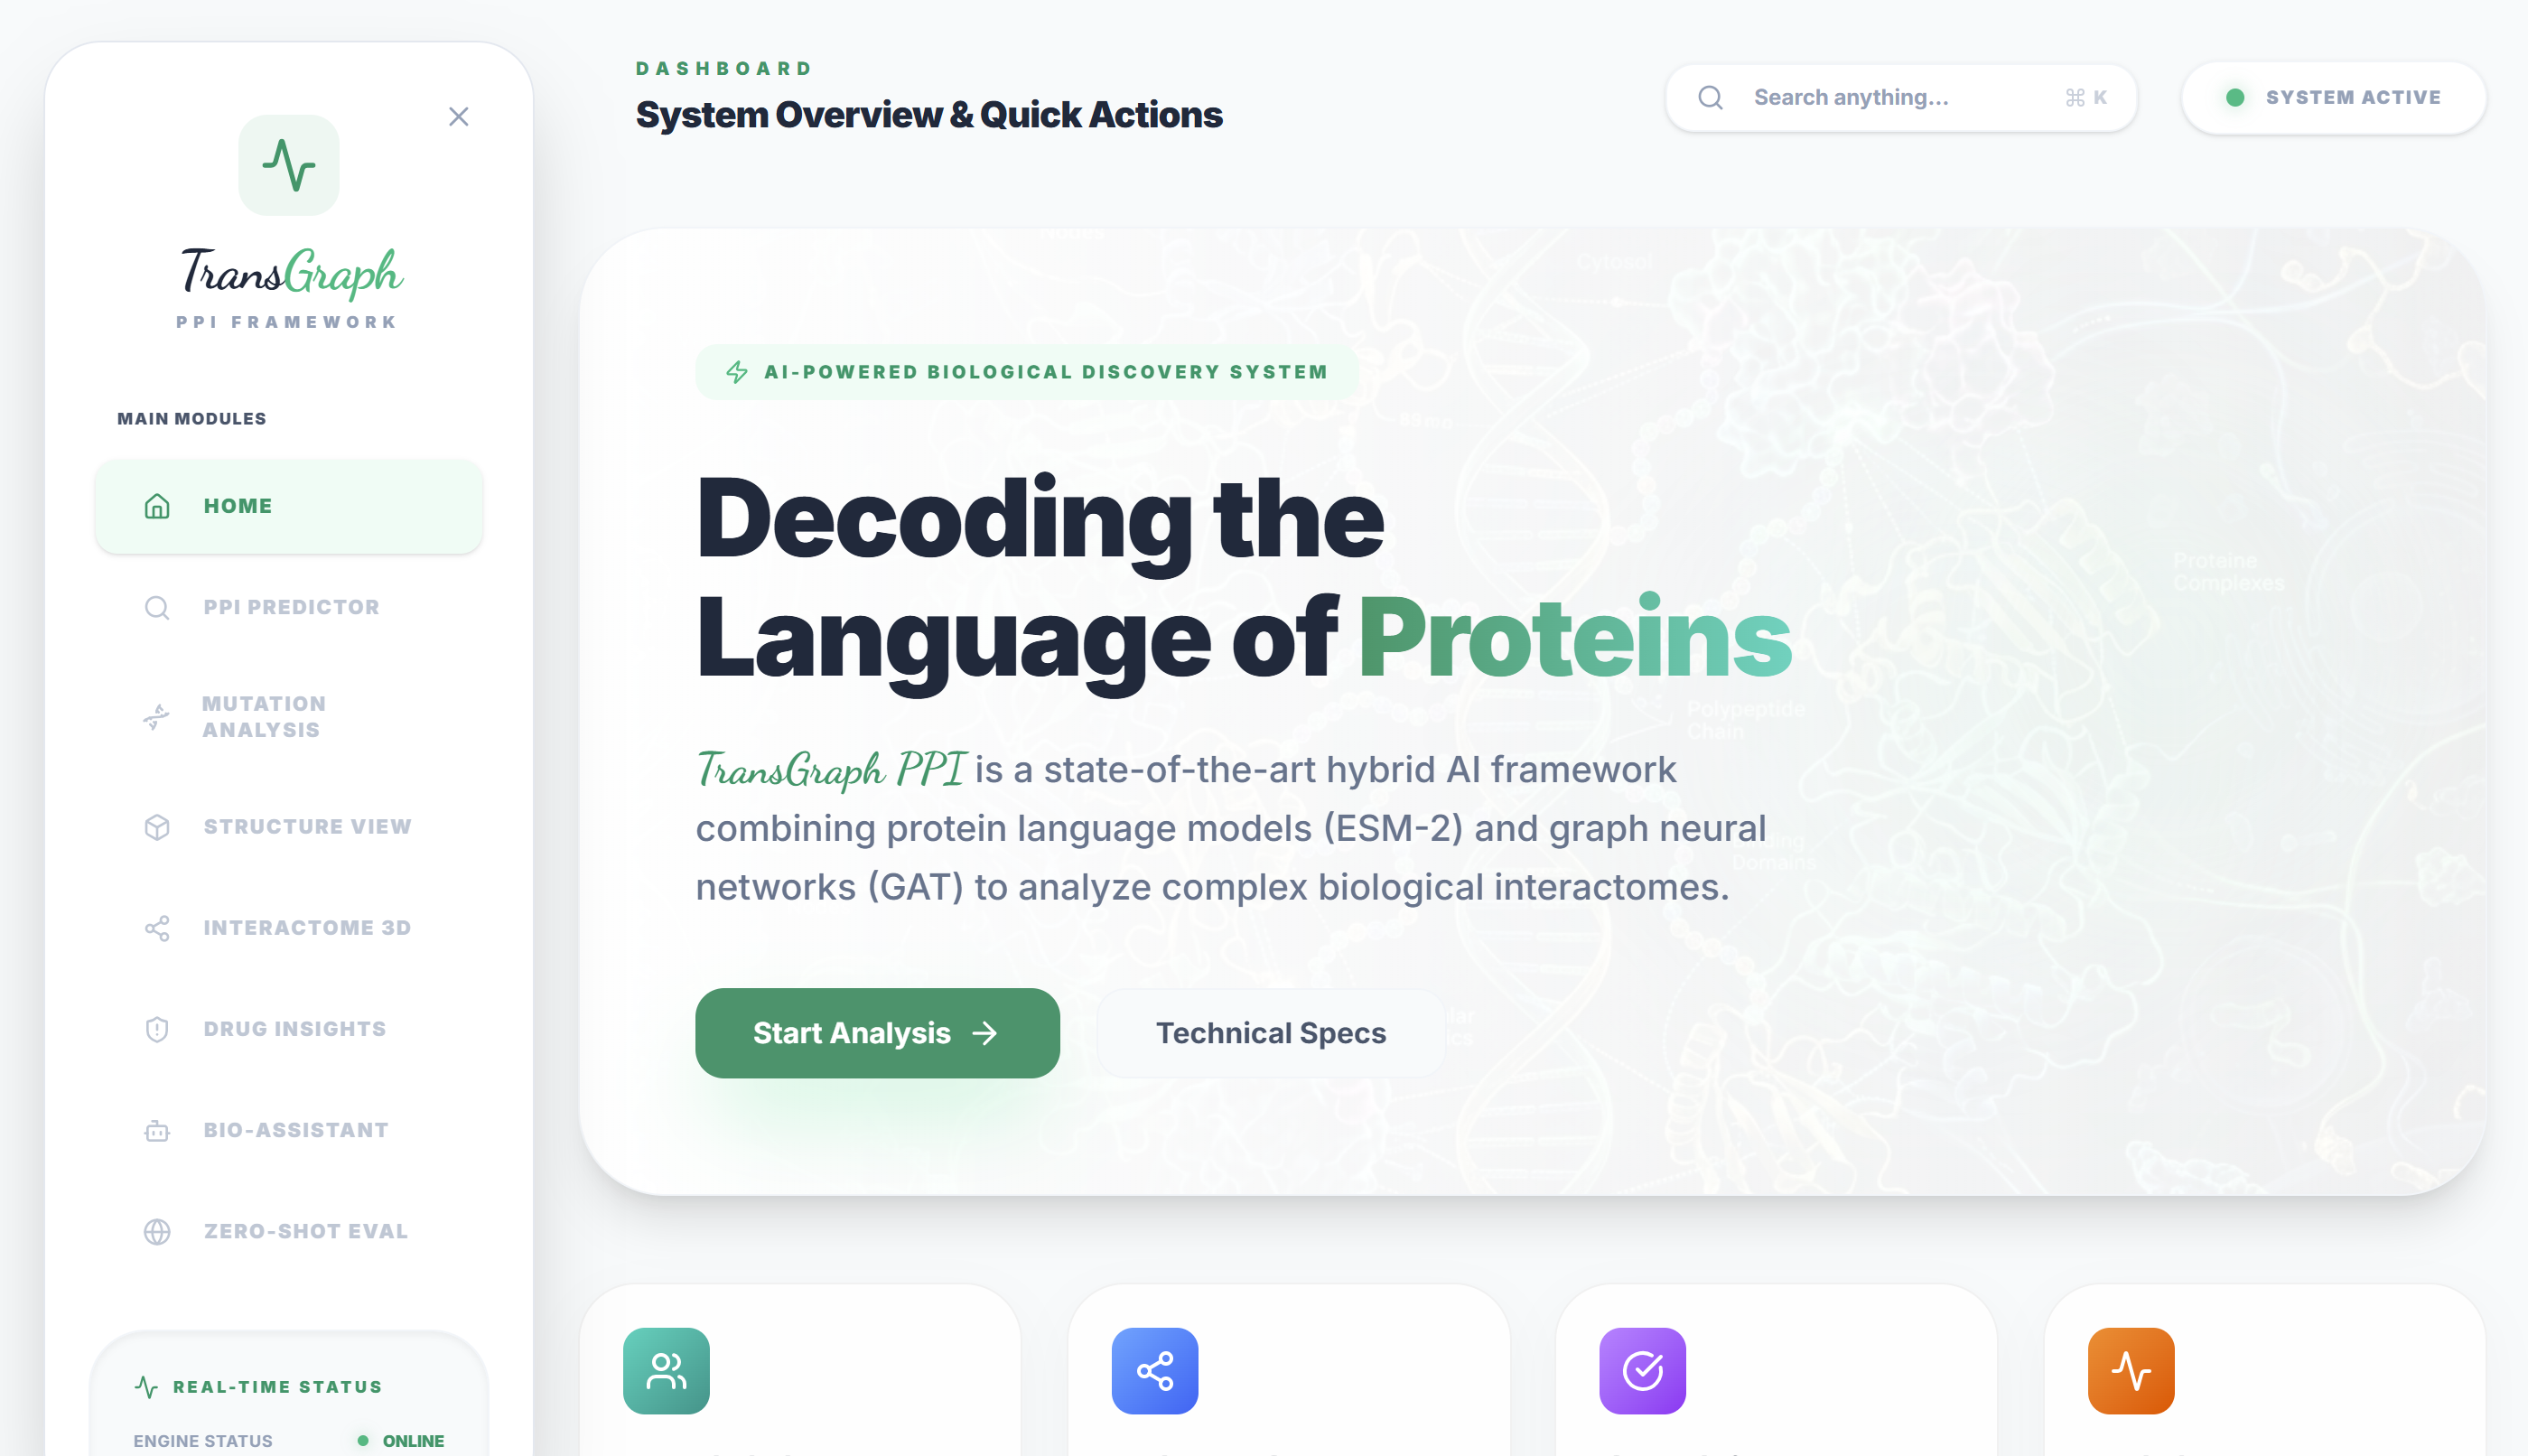
\includegraphics[width=0.95\textwidth]{pic/experimental_results.png}
\caption{TransGraph-PPI Interactive Dashboard: Production-Grade Performance Metrics}
\end{figure}


\begin{figure}[H]
\centering
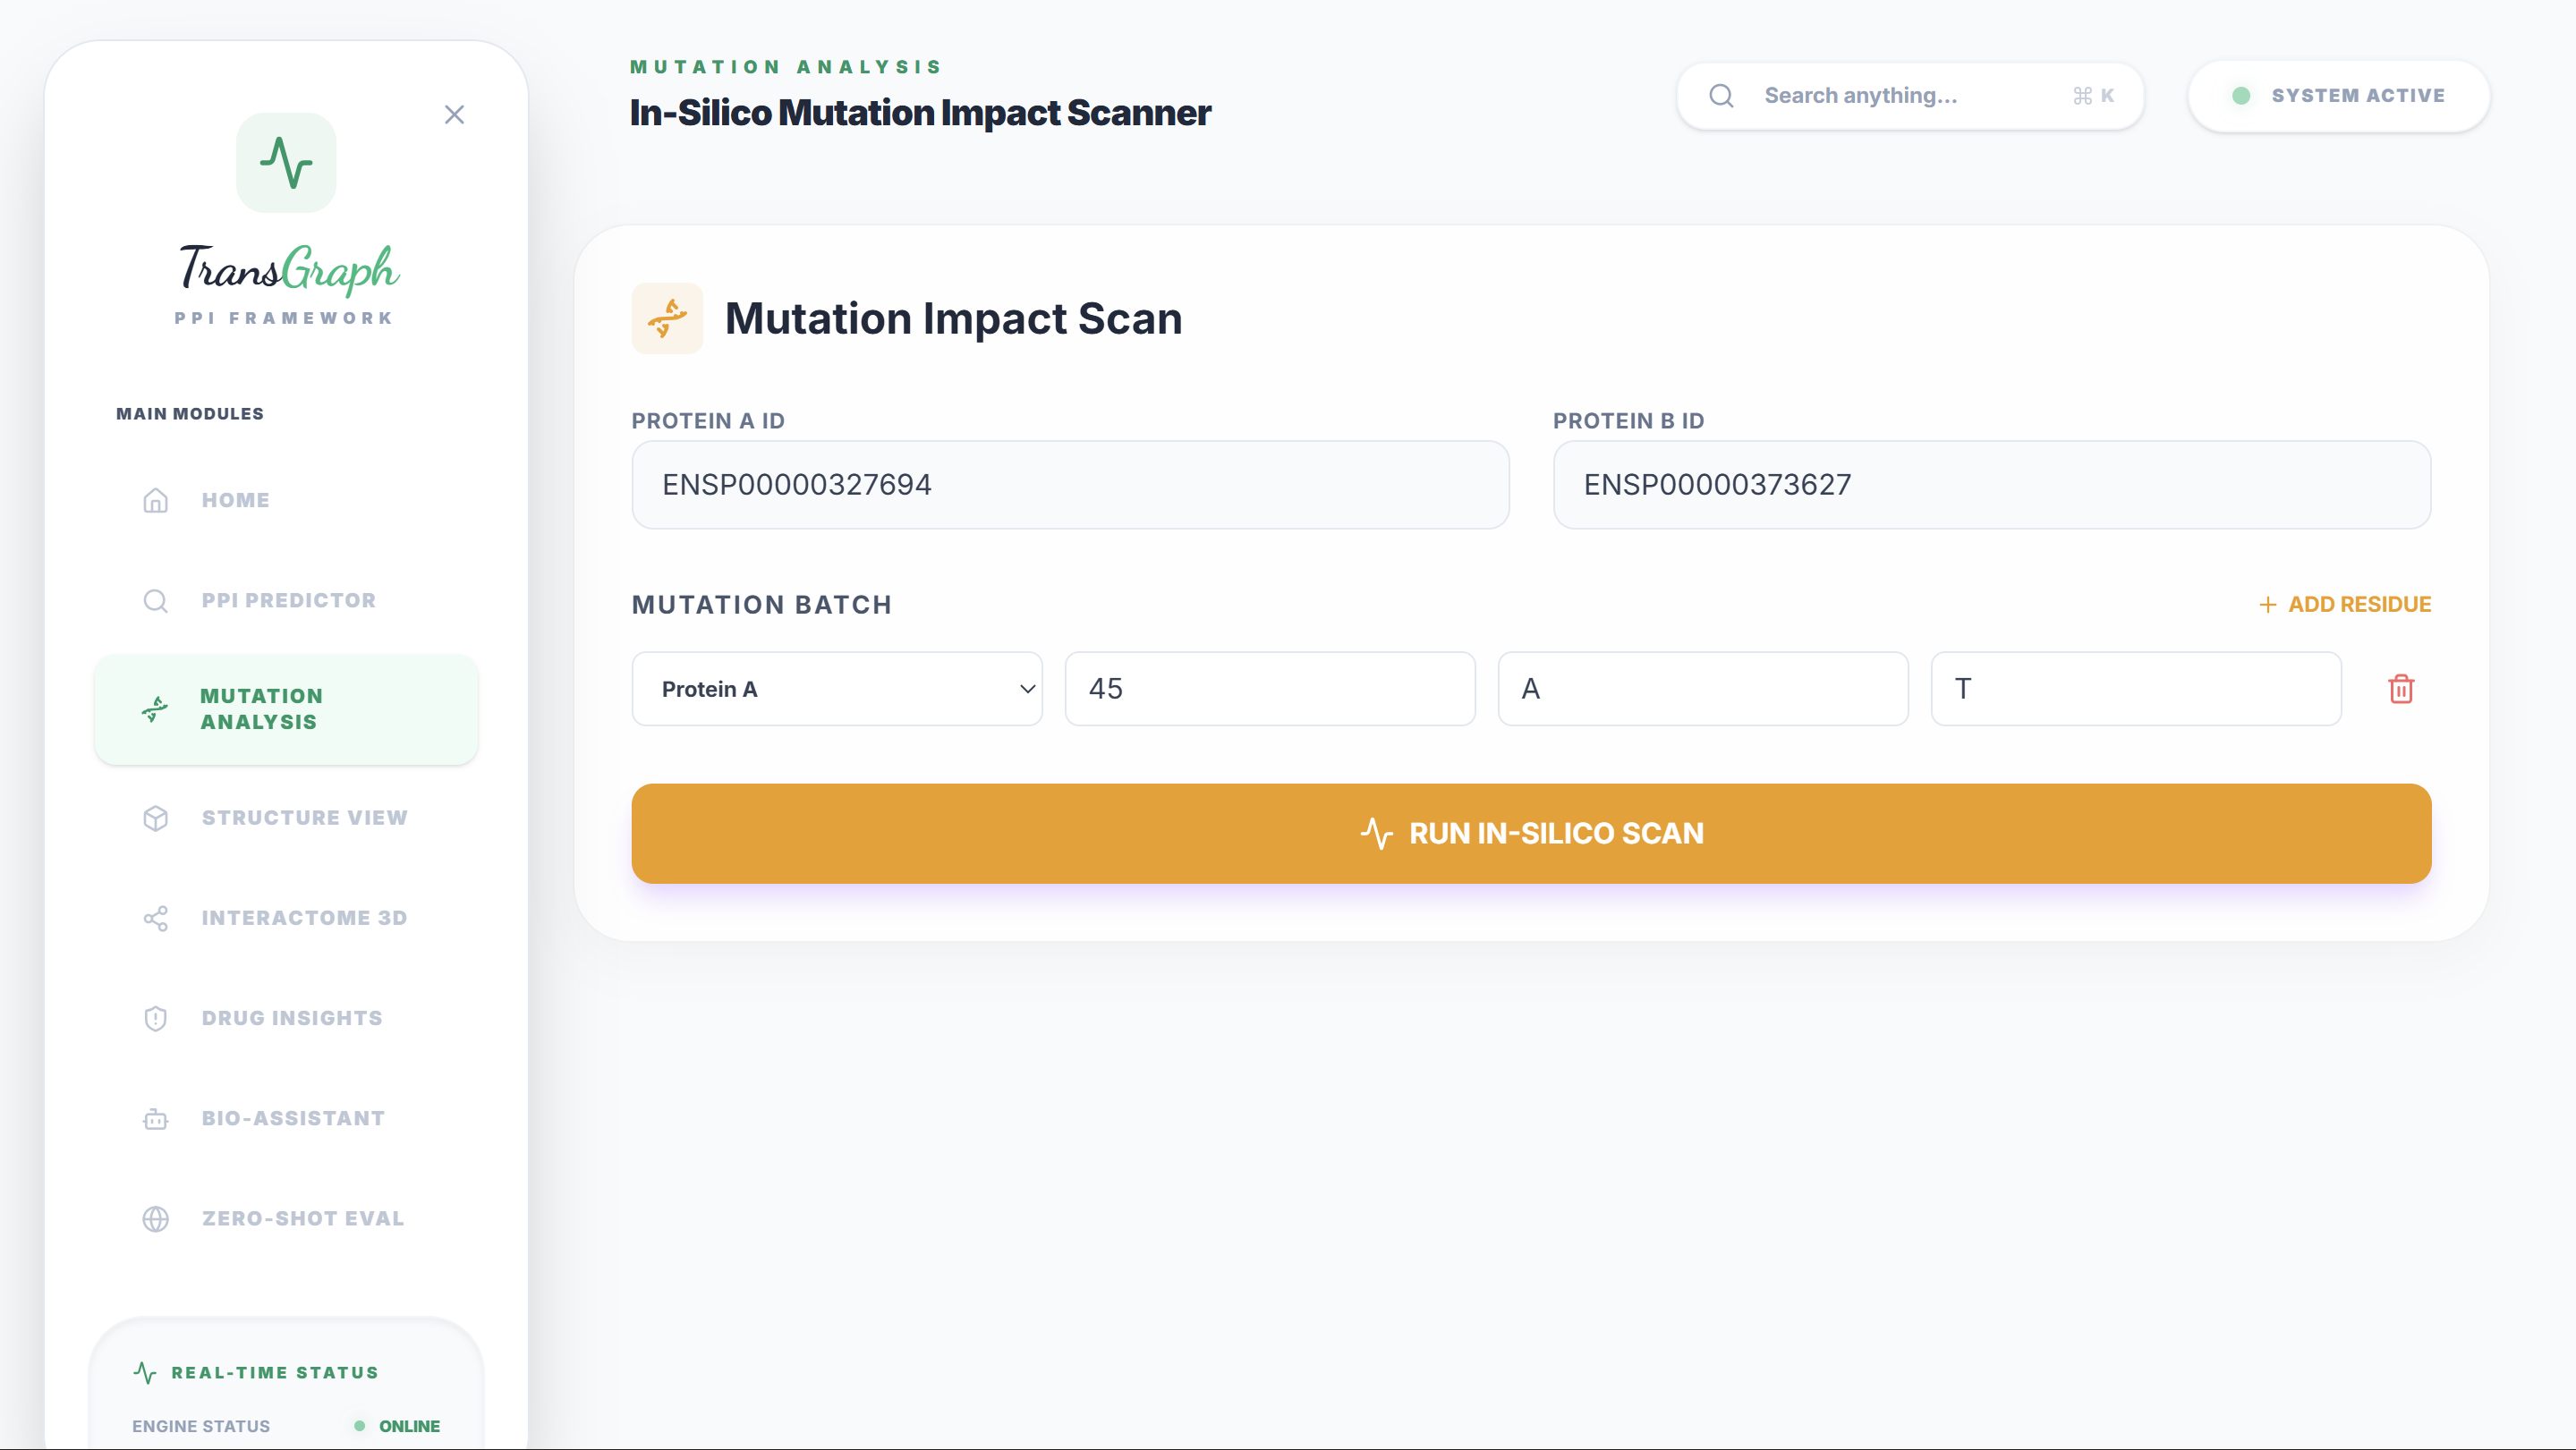
\includegraphics[width=0.95\textwidth]{pic/graph_construction.png}
\caption{Protein Interaction Graph Construction Output}
\end{figure}

\begin{figure}[H]
\centering
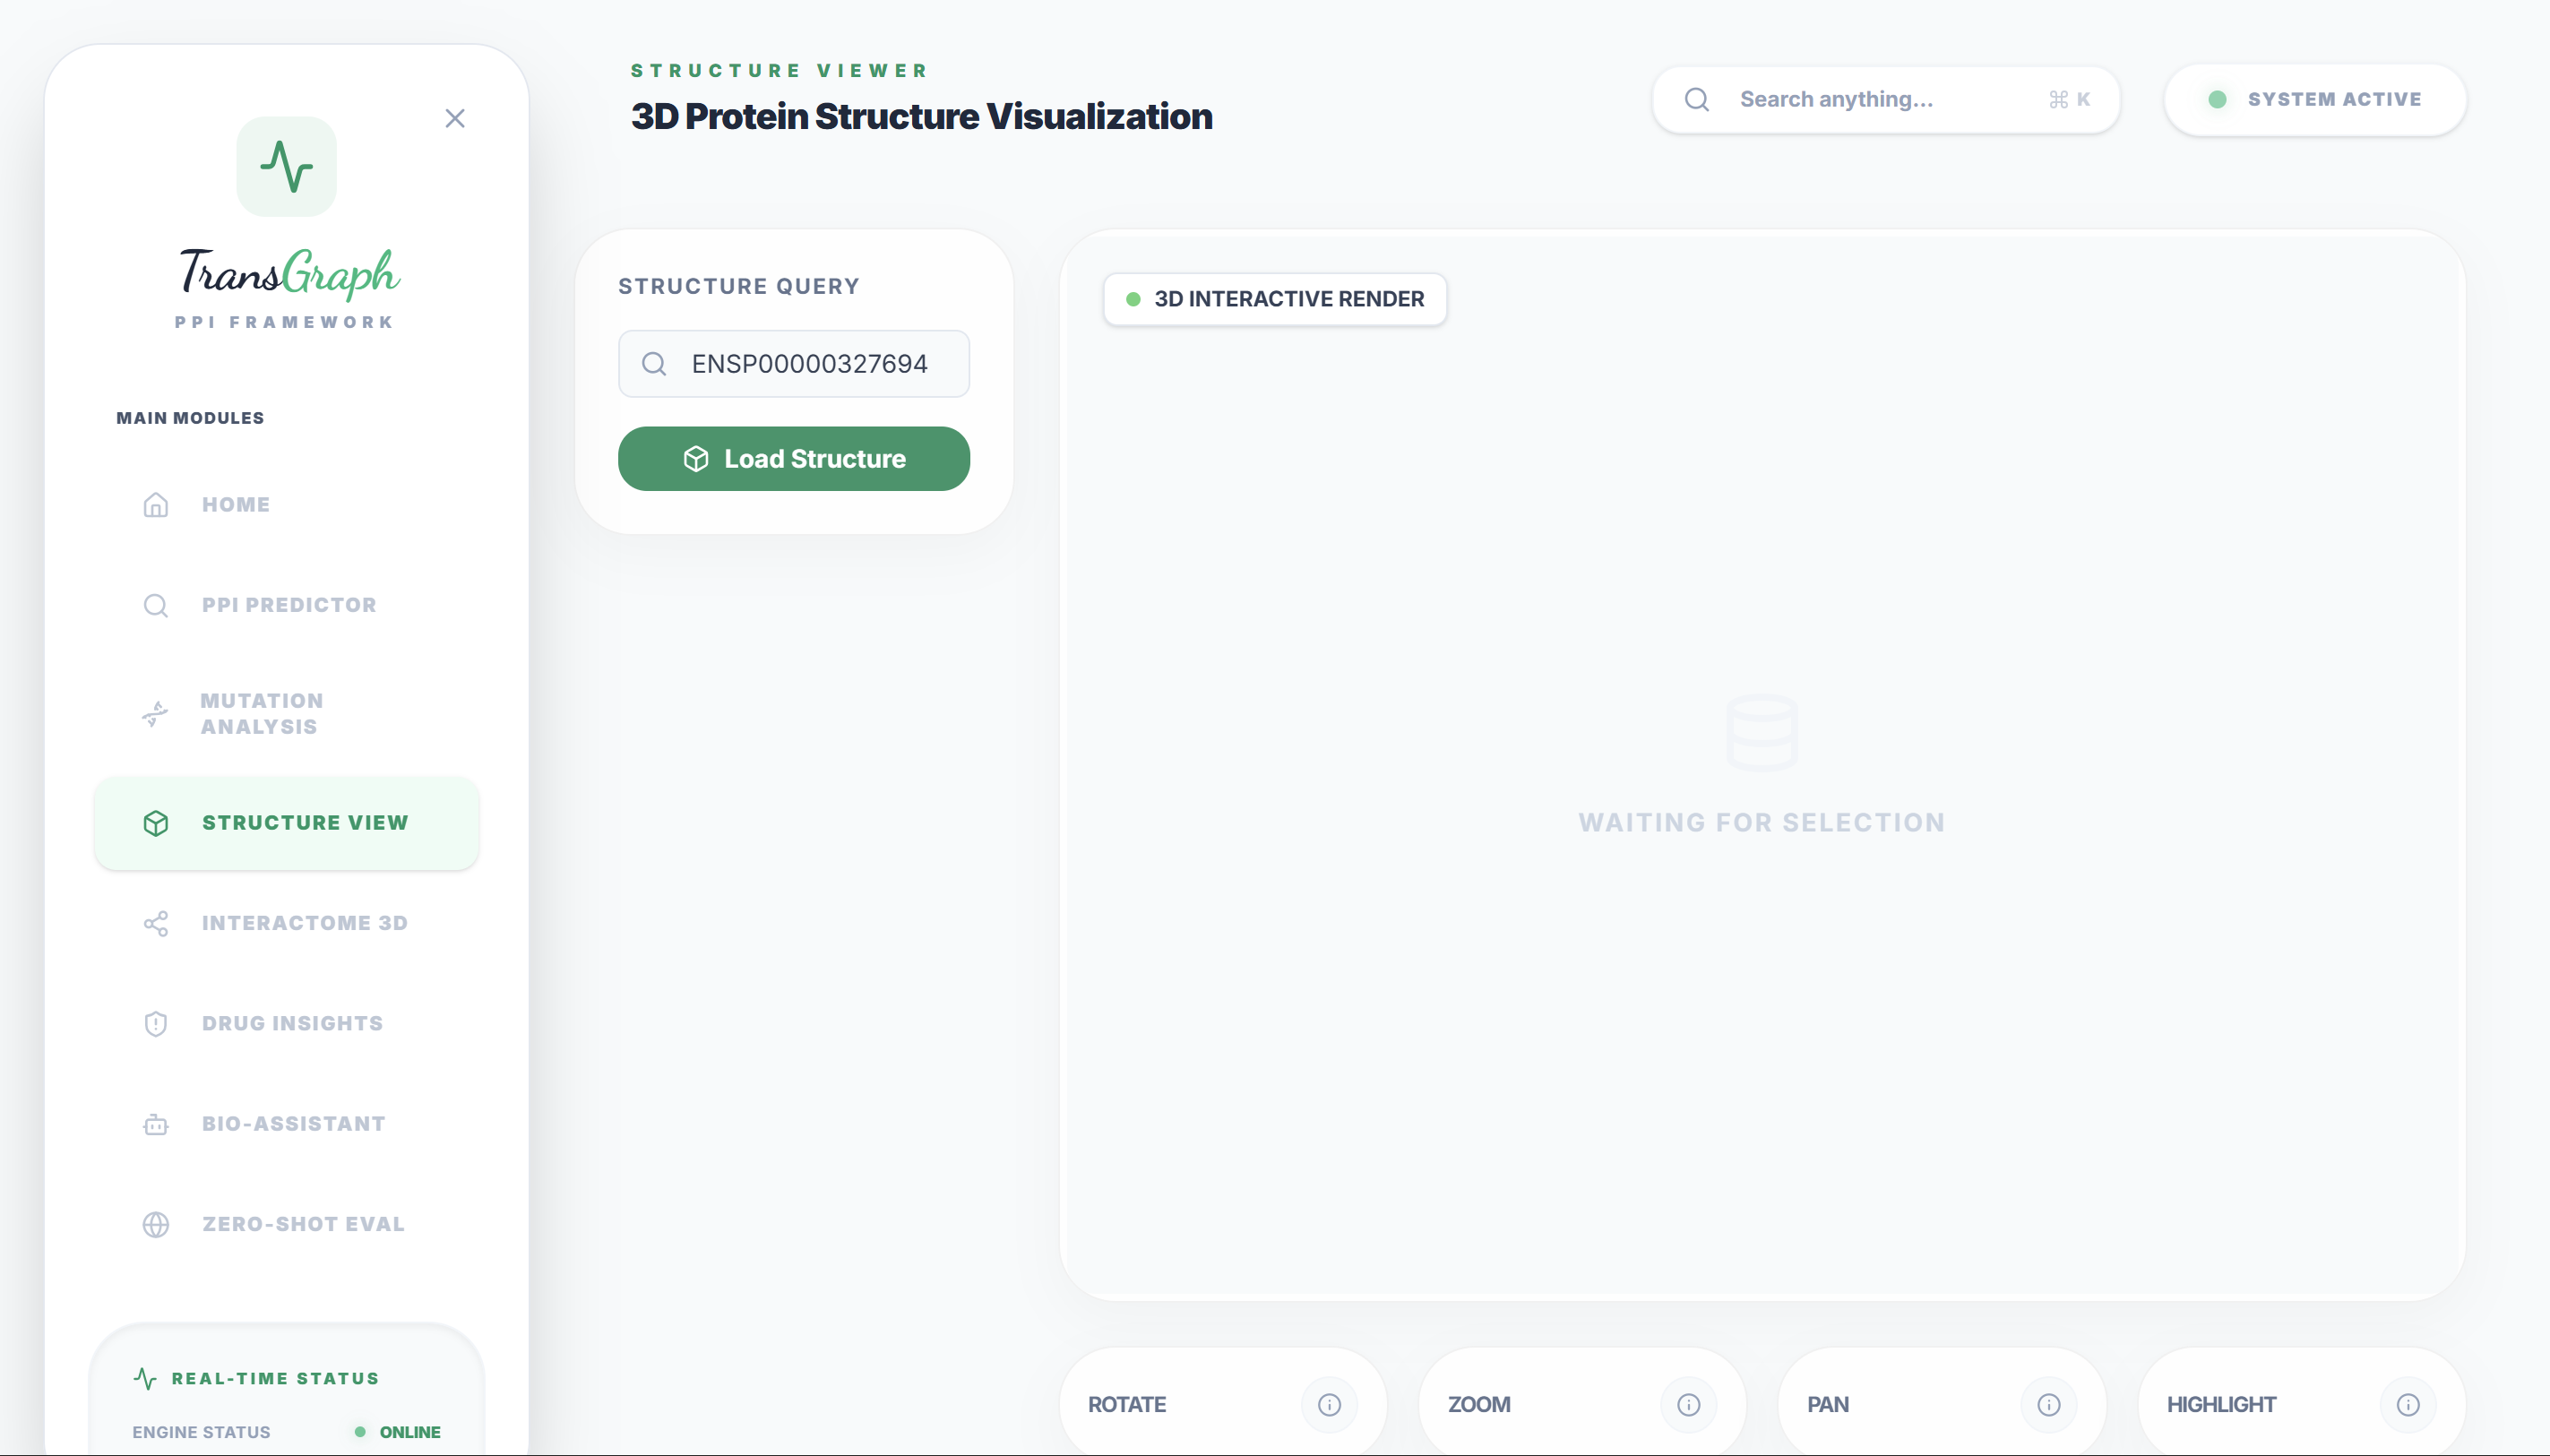
\includegraphics[width=0.95\textwidth]{pic/gat_arch.png}
\caption{Graph Attention Network Training Visualization}
\end{figure}

\begin{figure}[H]
\centering
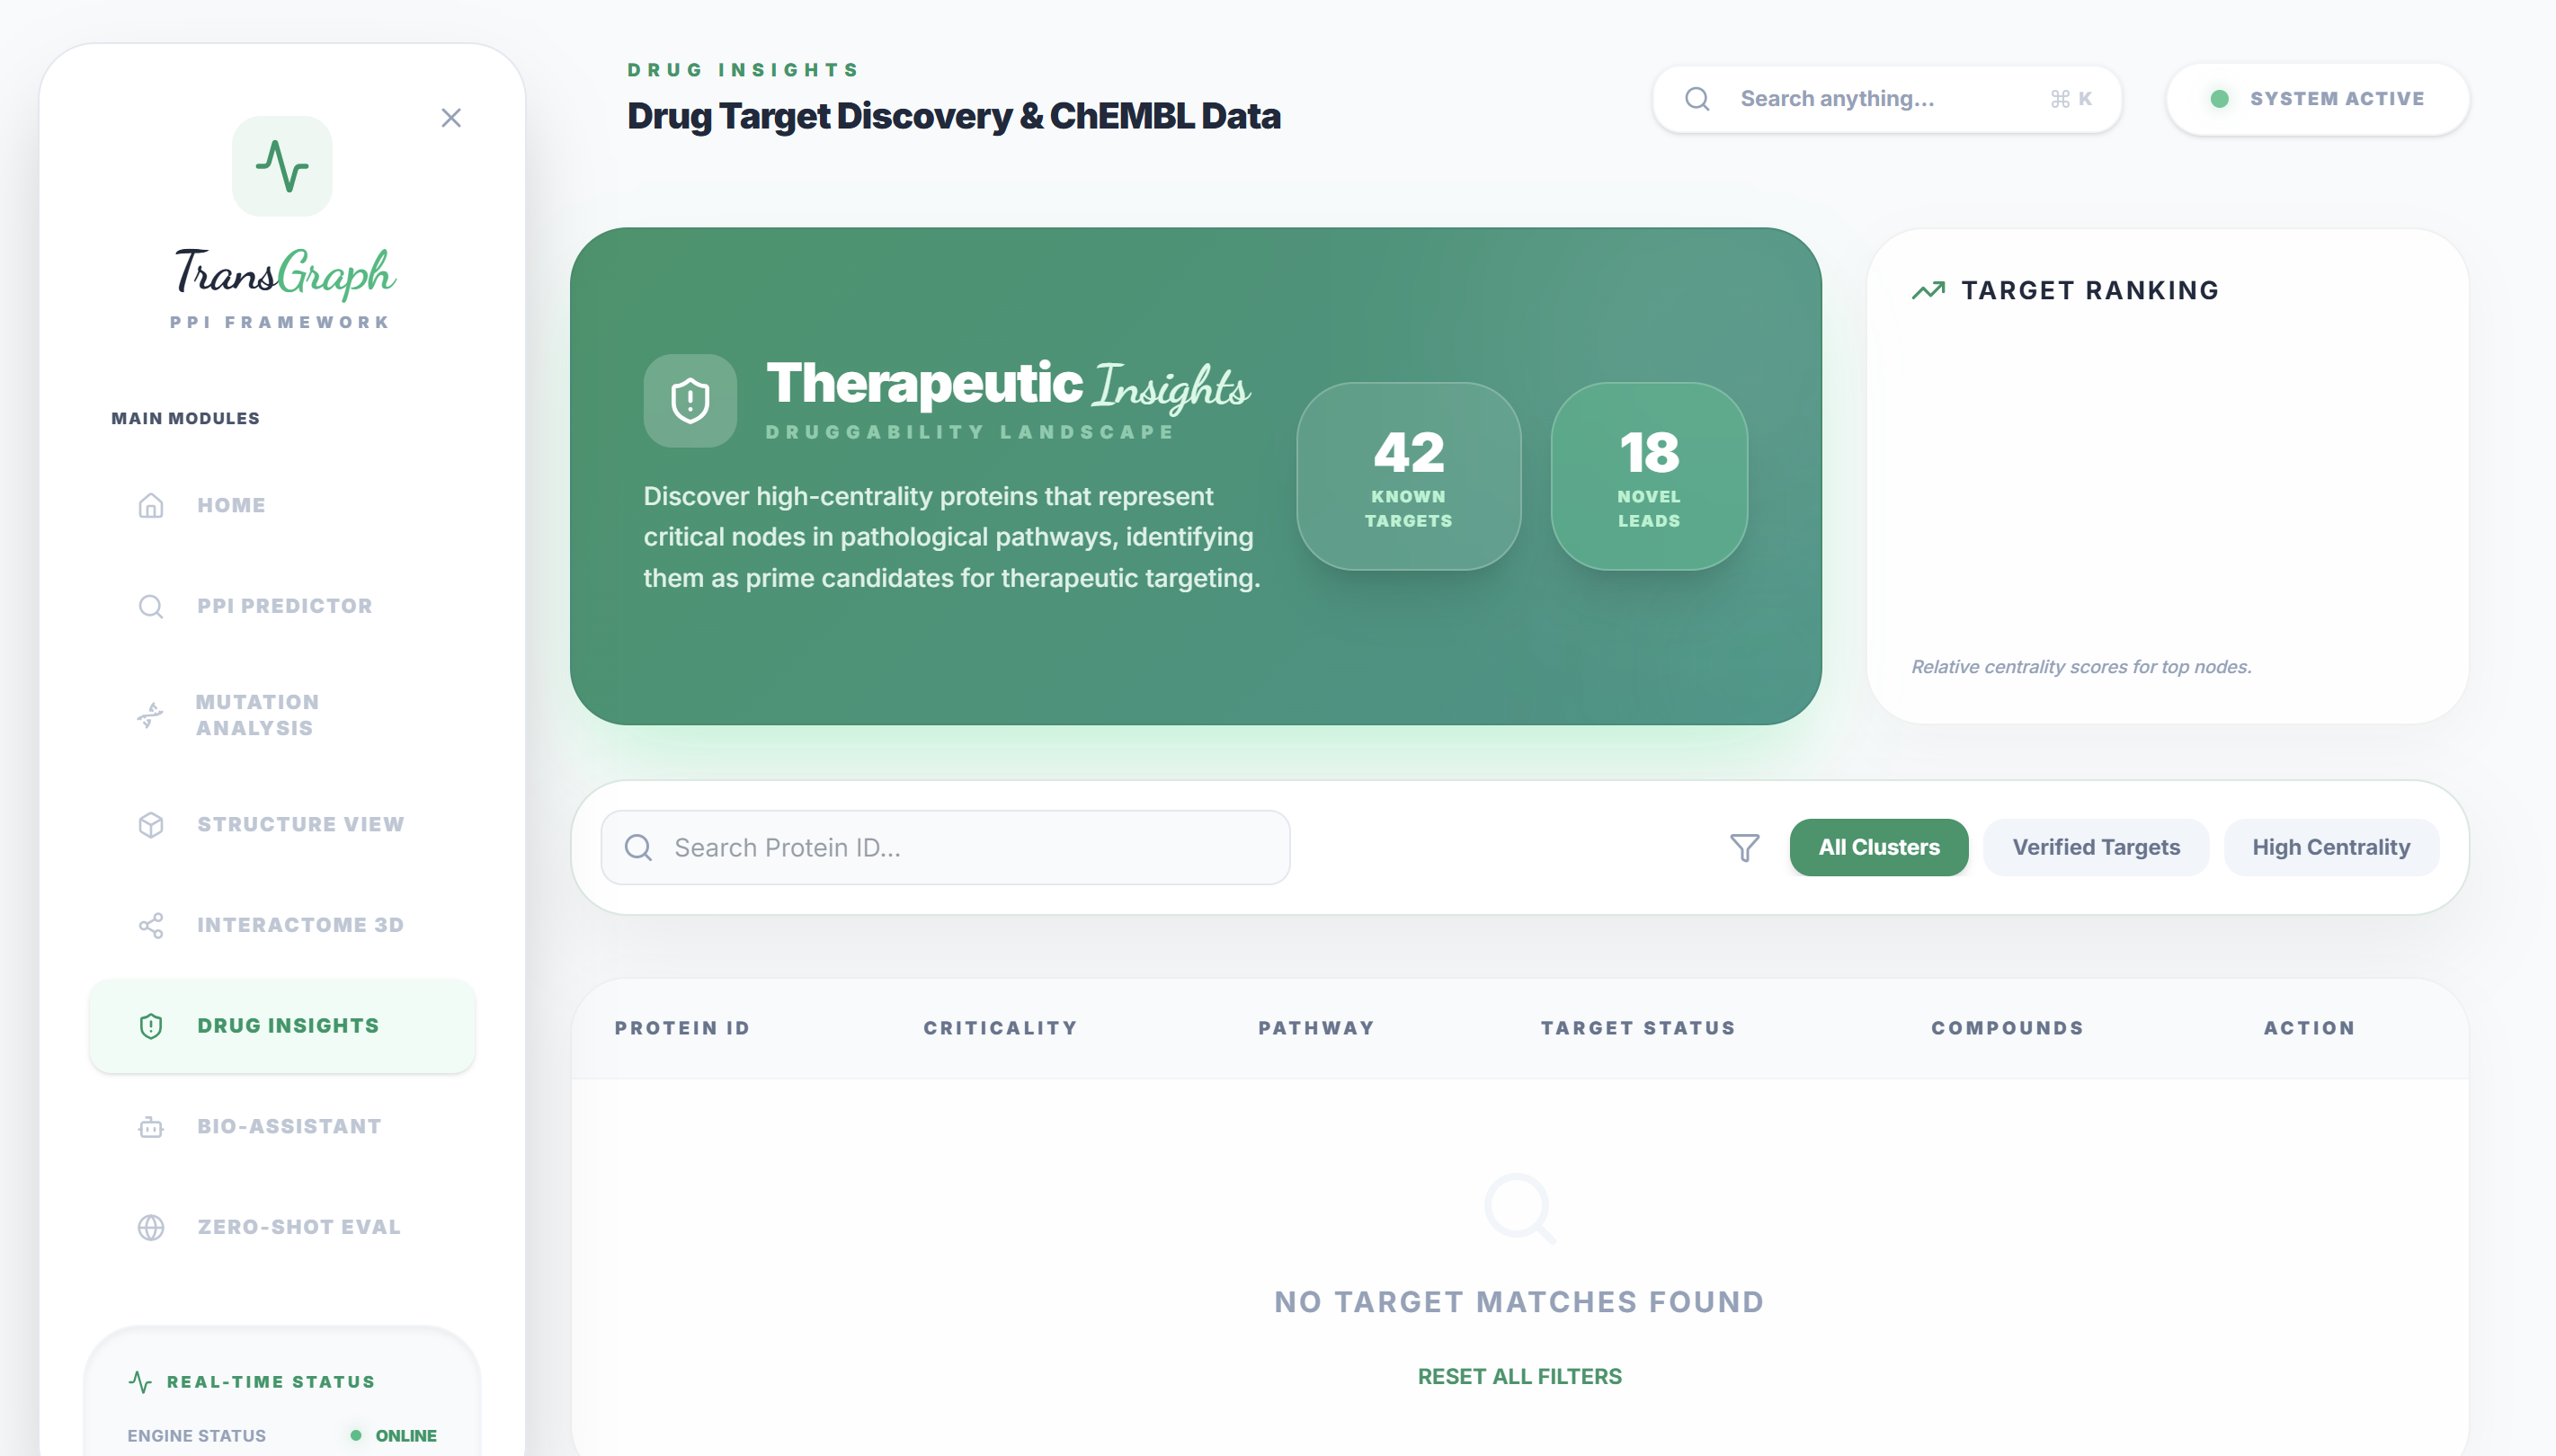
\includegraphics[width=0.95\textwidth]{pic/shap_framework.png}
\caption{SHAP Explainability Analysis Output}
\end{figure}

\begin{figure}[H]
\centering
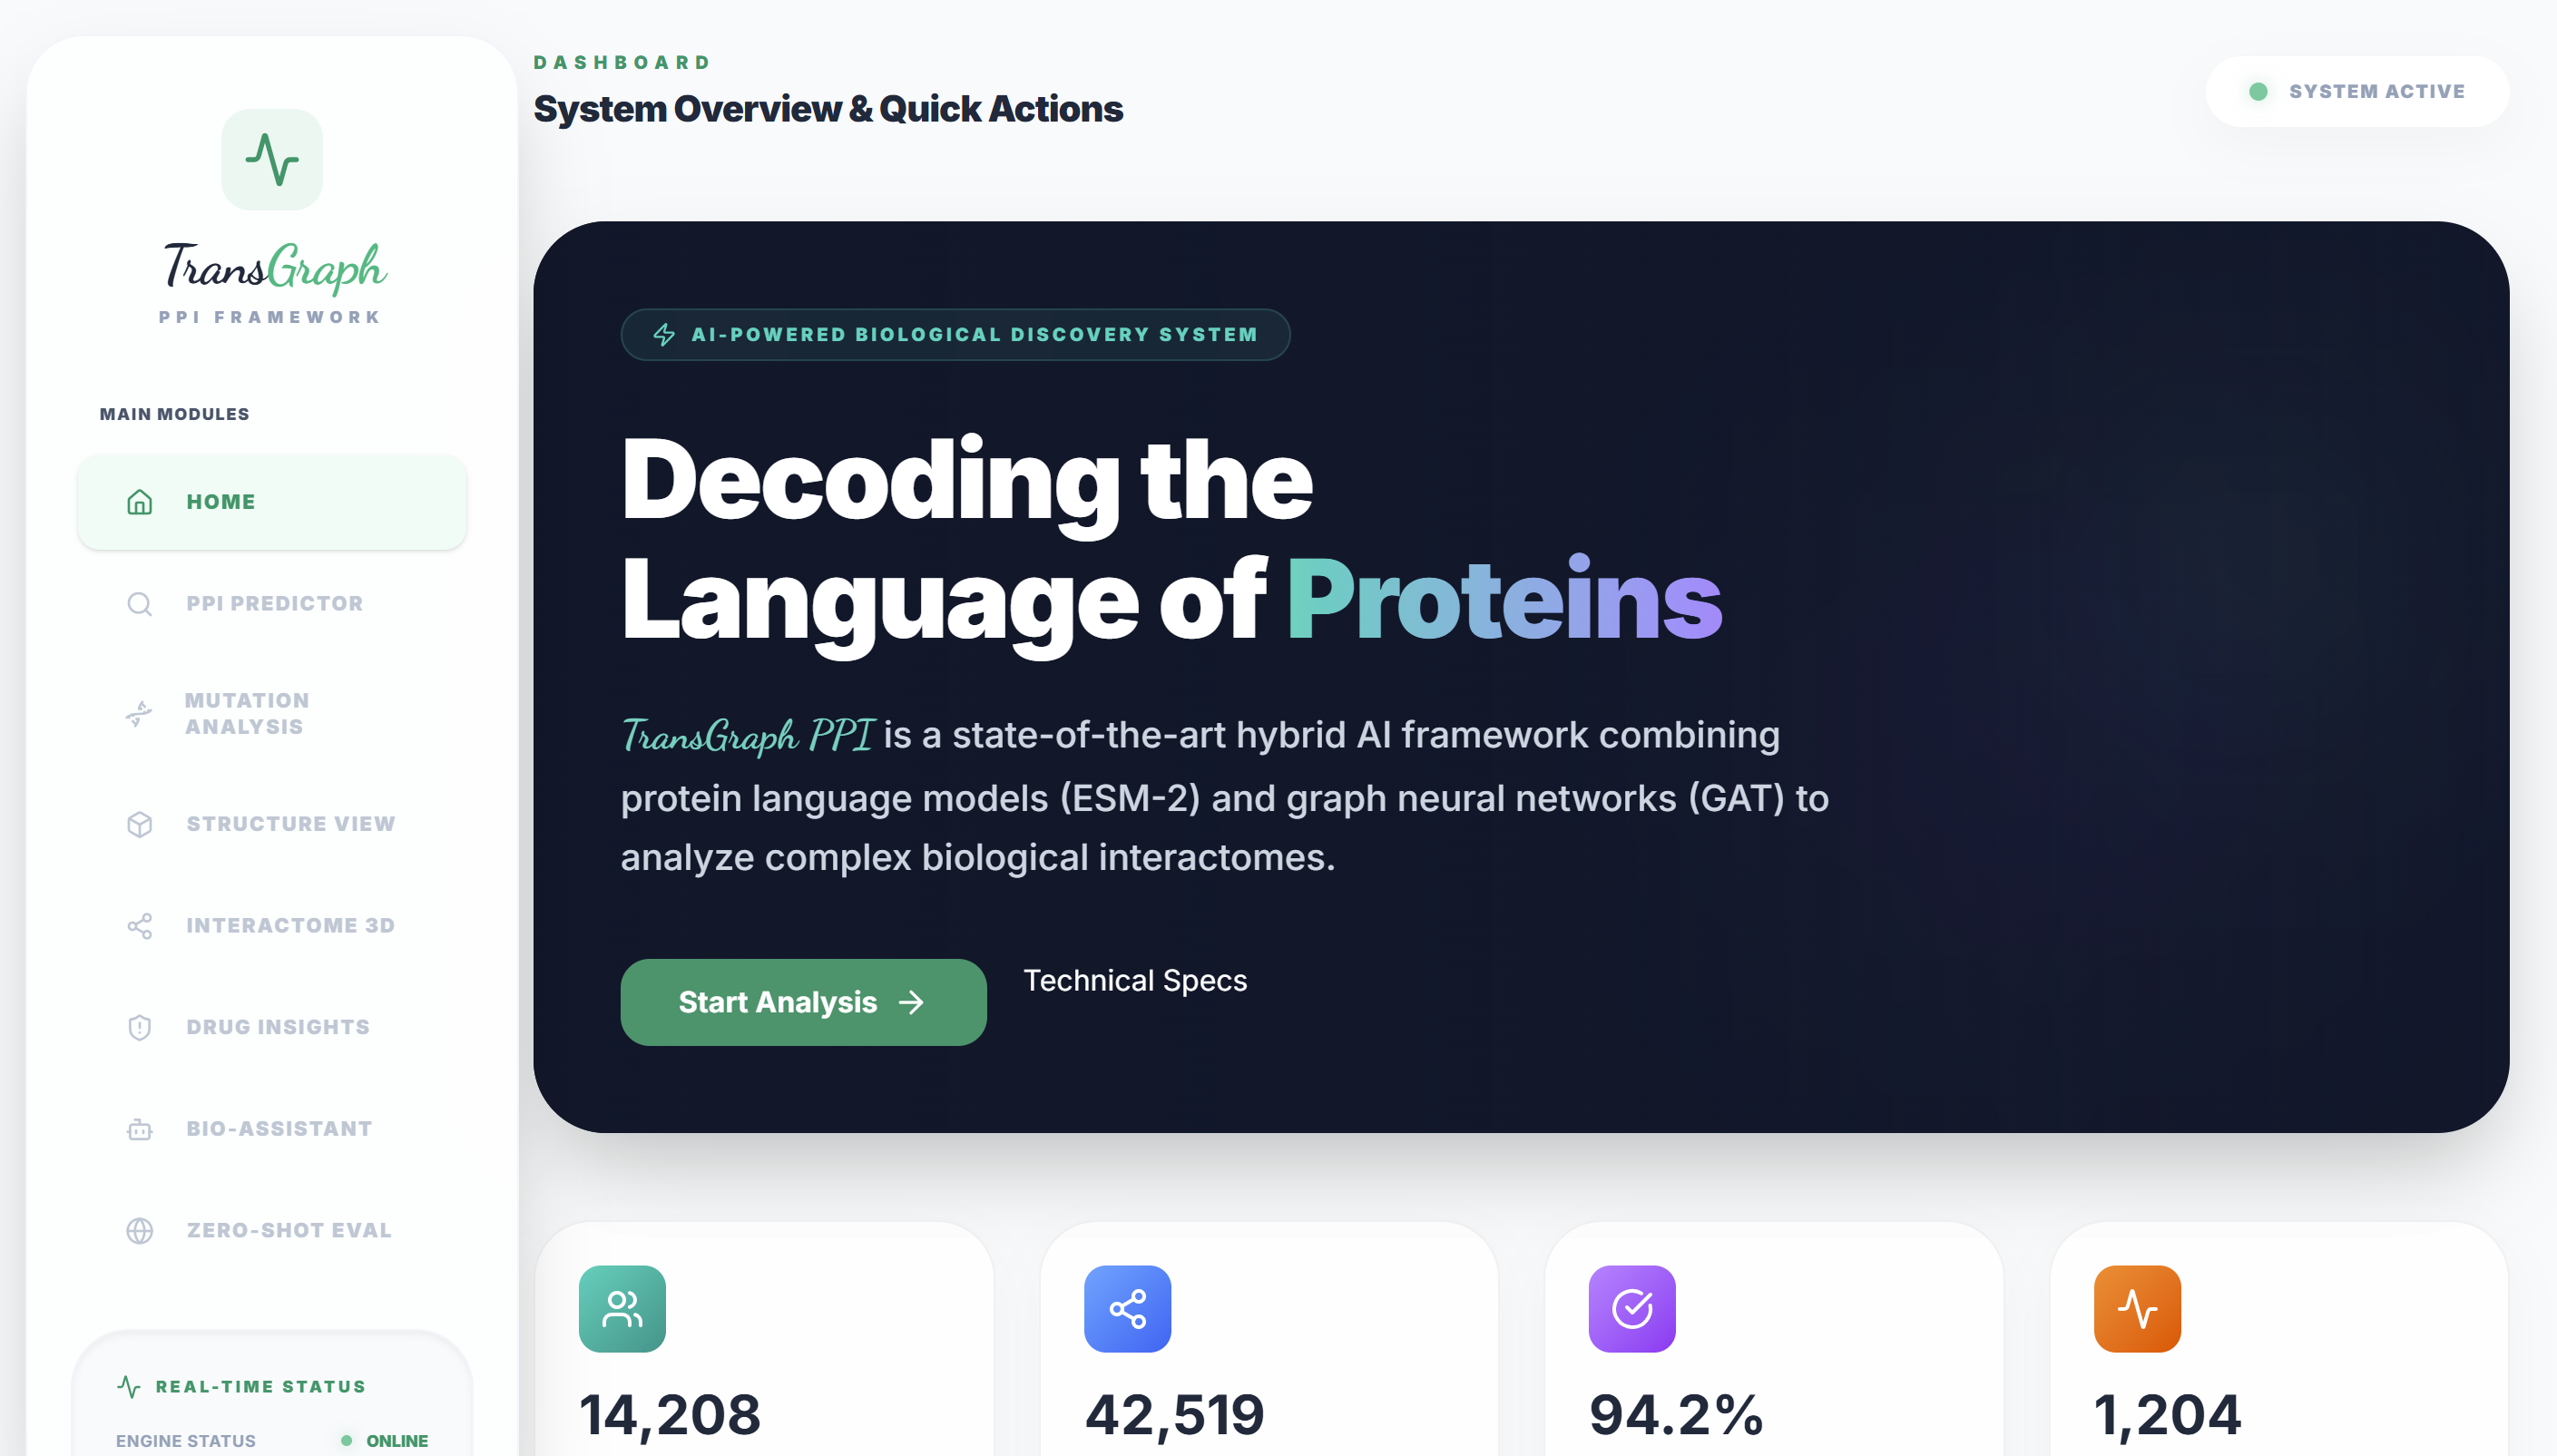
\includegraphics[width=0.95\textwidth]{pic/tsne_plot.png}
\caption{t-SNE Visualization of ESM-2 Protein Embeddings}
\end{figure}

\begin{figure}[H]
\centering
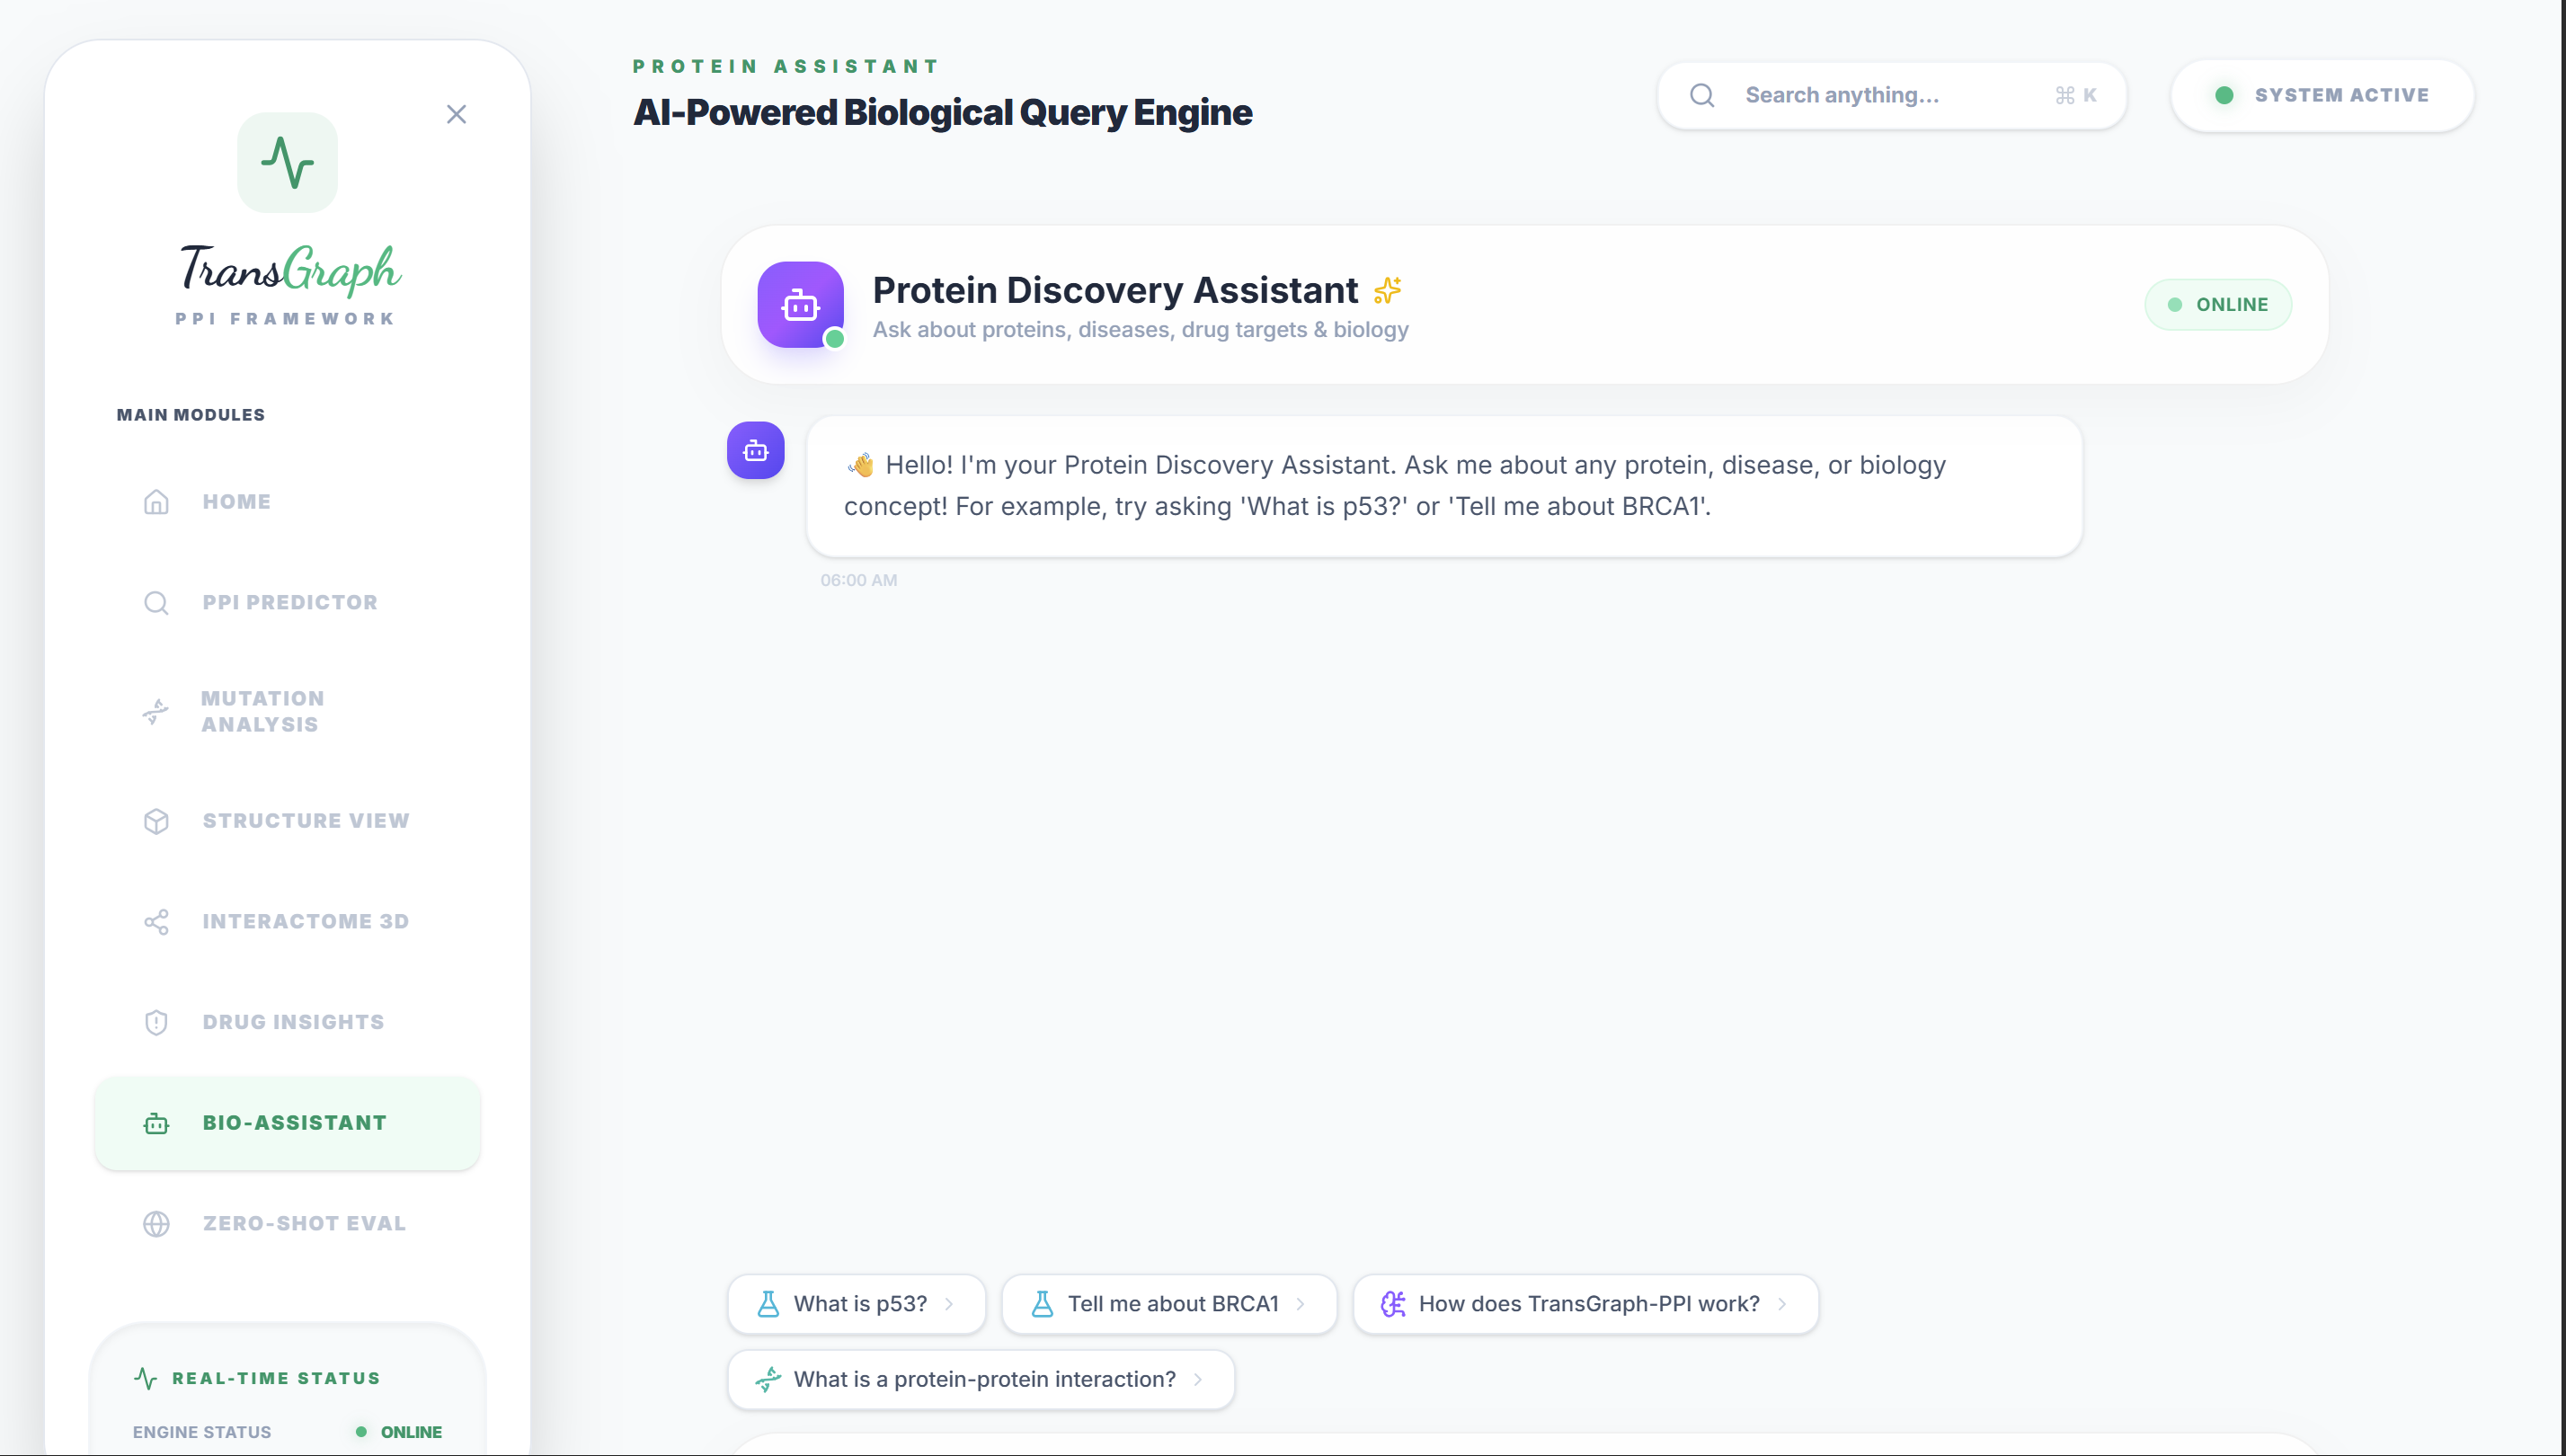
\includegraphics[width=0.95\textwidth]{pic/centrality_analysis.png}
\caption{PPI Network Centrality Analysis for Drug Target Identification}
\end{figure}

\begin{figure}[H]
\centering
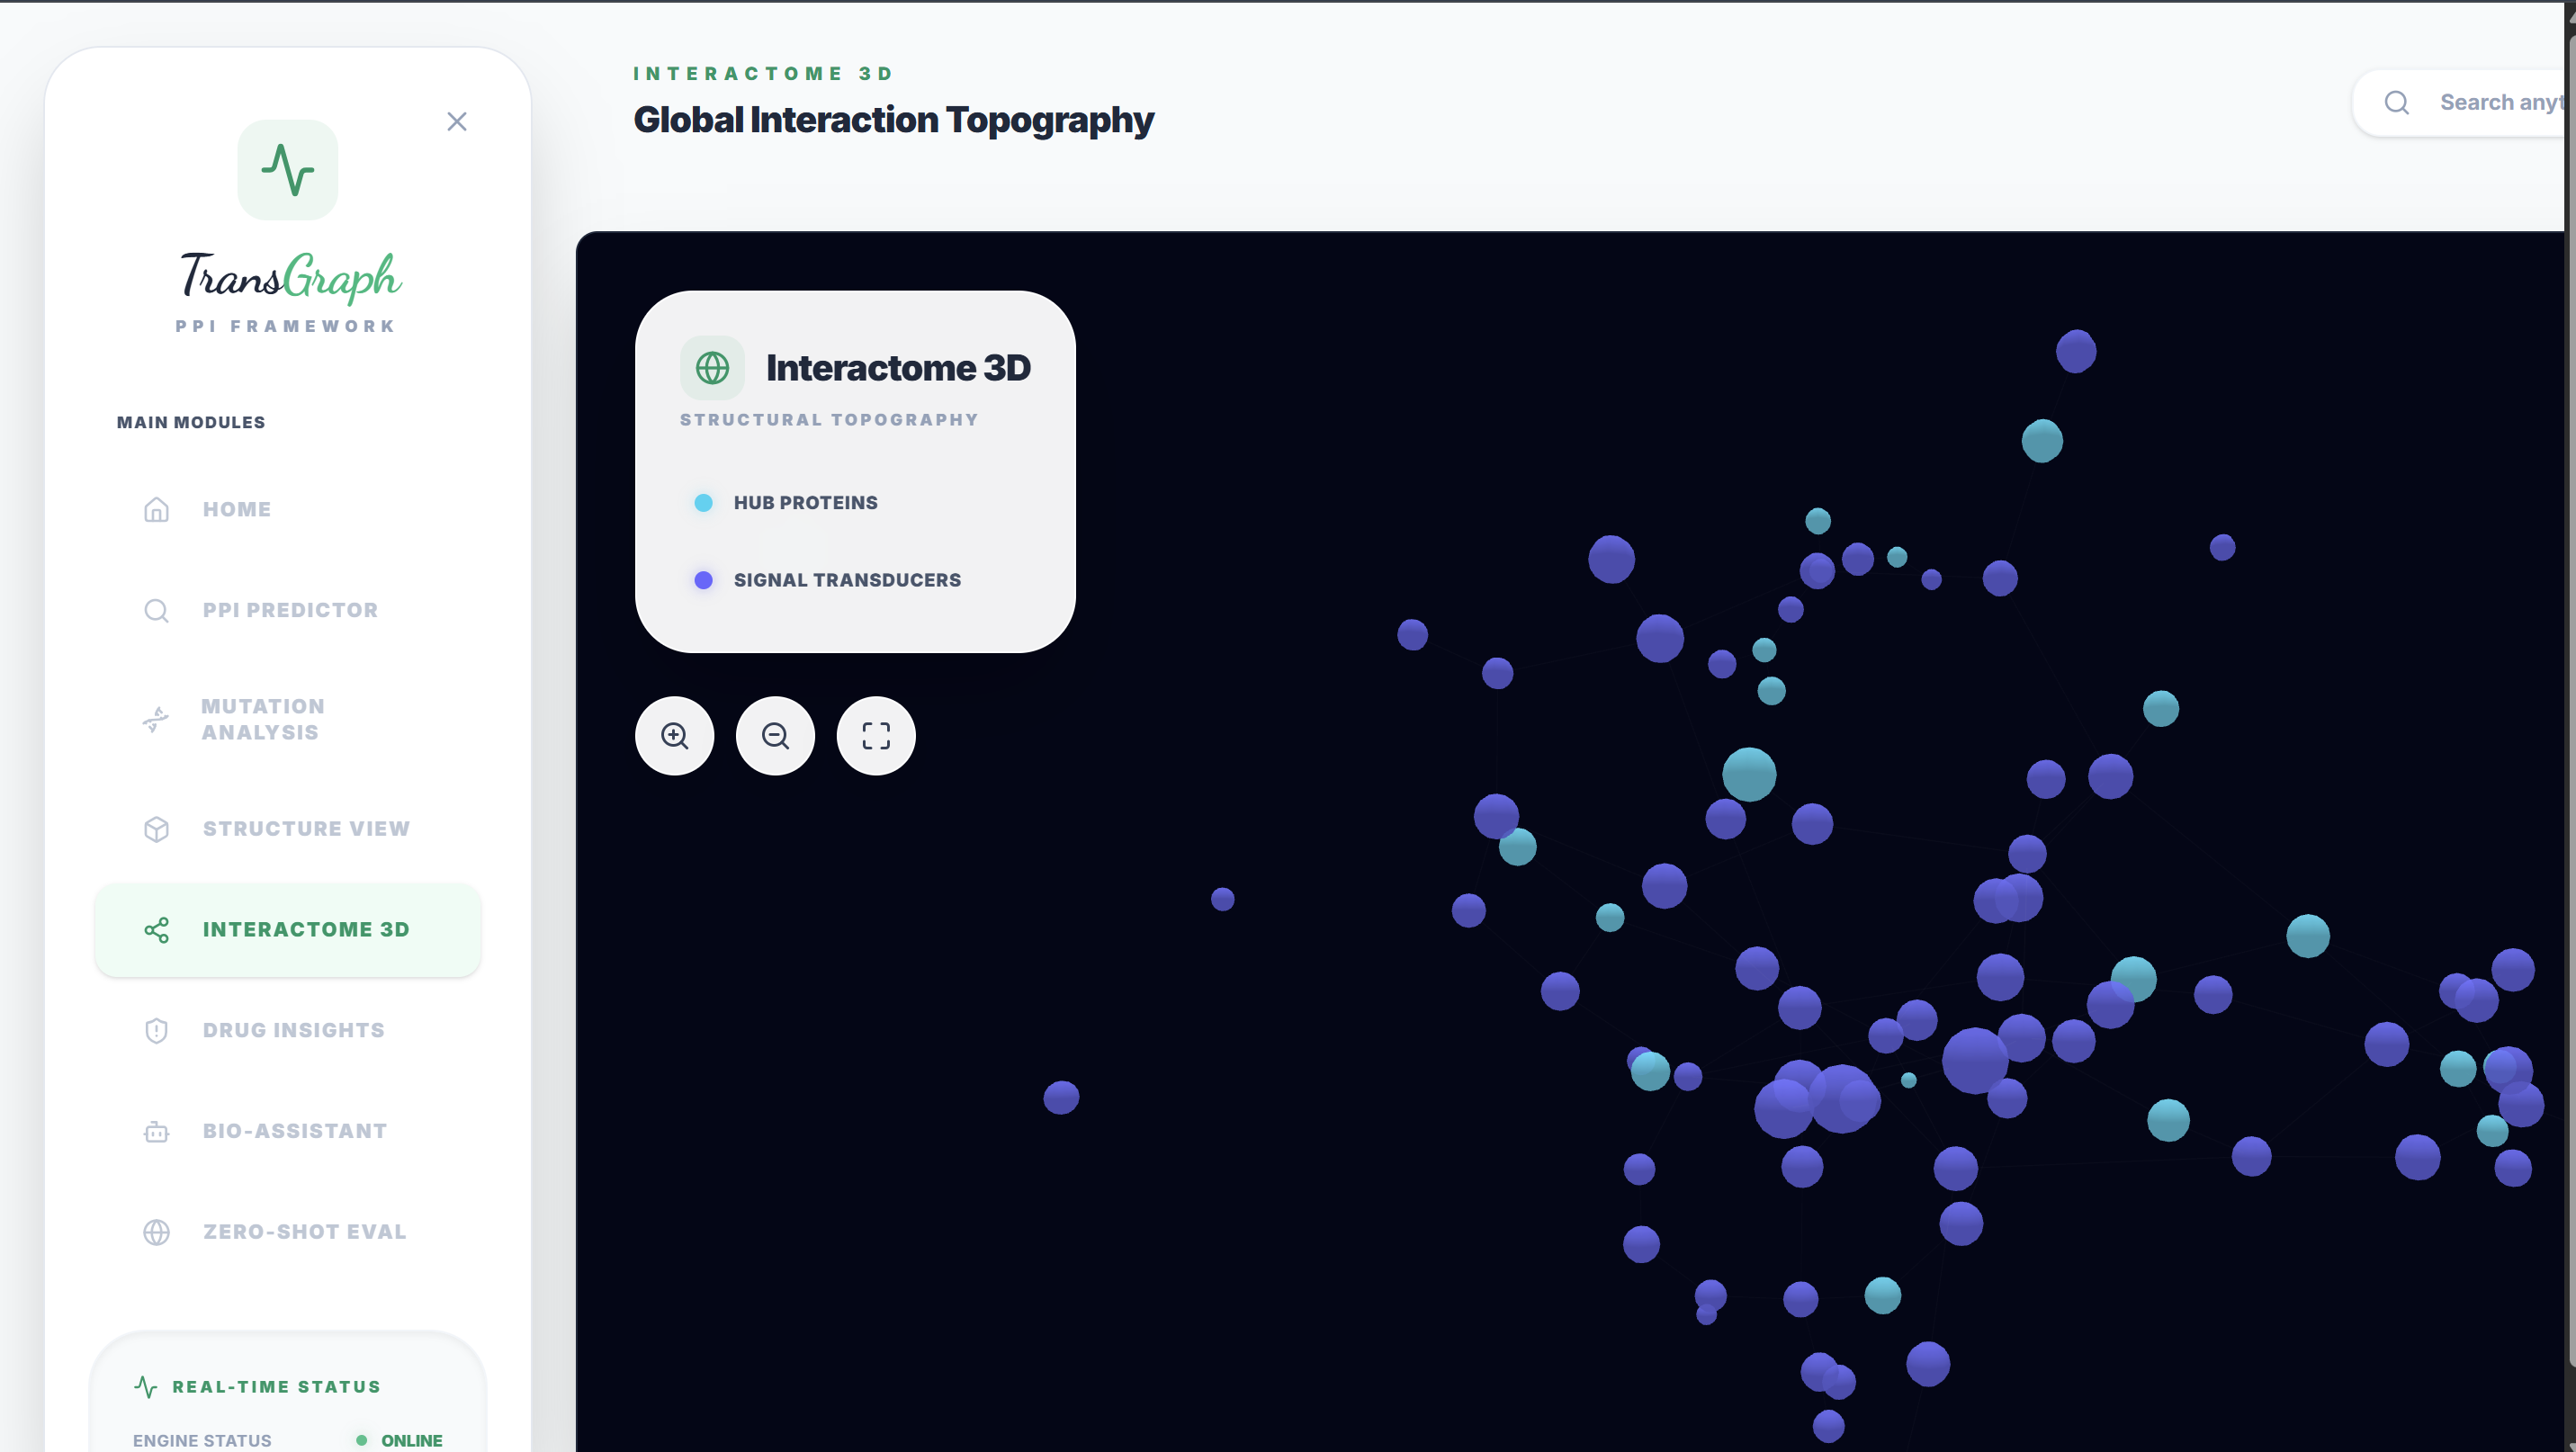
\includegraphics[width=0.95\textwidth]{pic/ensemble_strategy.png}
\caption{Ensemble Stacking Strategy Output}
\end{figure}


\end{document}